\section{Einleitung}
\label{sec:intro}
In den letzten Jahrzehnten folgte der Fortschritt der Rechenleistung dem Mooreschen Gesetz. Basierend auf der Miniaturisierung von Transistoren verdoppelte sich die Hardwareleistung für von-Neumann-Architekturen alle 18 Monate. So wurde die Lösung von schwierigen Optimierungsproblemen vorangetrieben, aber physikalische Gesetze begrenzen diese Entwicklung, wenn die Chip-Größe bei atomarer Skala ankommt.
Dies erfordert einen neuen Ansatz: Quantum Computing \cite{Colwell2013}.\\
Unsere Aufgabe für die \textit{QC-Optimization-Challenge} des \textit{QAR-Lab} wurde von dem Unternehmen TRUMPF bereitgestellt:
Es handelt sich um ein flexibles Job-Shop-Scheduling-Problem (JSSP) aus der Blechfertigung. Für aus Rohblechen geschnittene Kleinteile muss zur Weiterverarbeitung eine richtige und effiziente Maschinenbelegung gefunden werden. Dieses Kombinationsproblem ist NP-hart\footnote{Da das bekannteste NP-harte Problem (Travelling Salesman Problem) eine simple Instanz eines JSSPs ist, folgt, dass unsere Problemstellung ebenfalls NP-hart ist.} weshalb es nicht in polynomieller Zeit, deterministisch  gelöst werden kann.
Das bedeutet, dass solch eine Problemstellung auch mit modernen Computern lediglich approximativ lösbar ist.\\
Daher stellt sich die Frage, wie man diese Problemstellung in der Zukunft effizient lösen kann. Hierzu untersuchen wir im Nachfolgenden den Einsatz von Quantencomputern.

\section{Grundlagen}
\label{sec:basics}
Als flexibles JSSP gehen wir im Nachfolgenden näher auf die Komplexität und Struktur des Problems ein. Im Anschluss erklären wir die quantenmechanischen Grundlagen für das Quantencomputing und gehen dann auf die einzelnen Teilbereiche -- Annealing und Gate Model -- ein.

\subsection{Job Shop Scheduling Probleme}
\label{subsec:jssp}
Der Begriff Job-Shop-Scheduling-Problem beschreibt eine Problemklasse in der ein Set von Jobs einem Set von Maschinen zugeordnet werden muss und dabei die sogenannte \textit{makespan} -- die Zeitspanne in der alle Jobs abgearbeitet werden -- so kurz wie möglich gehalten werden soll.
Ein Job besteht dabei aus ein oder mehreren Operationen eines oder mehrerer Operationstypen, wobei diese unterschiedlich lange Durchführungzeiten haben und einer Operationsreihenfolge unterliegen.
Schließlich hat jeder Job noch eine individuelle Deadline zu der alle seine Bauteile abgearbeitet sein sollen. In unserem Fall hat jede Maschine einen Operationstyp und kann zu jedem Zeitpunkt maximal eine Operation dieses Operationstyps ausführen\cite{Venturelli2016}.
\begin{figure}[H]
	\centering
	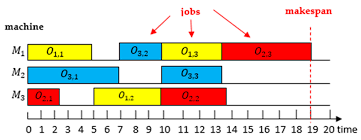
\includegraphics[scale=0.5]{images/JSSP.png}
	\caption{JSS-Problembeispiel mit drei Jobs und drei Maschinen}
	\label{figure:JSSP-Beispiel}
\end{figure}
Bei unserer Problemstellung handelt es sich um den Spezialfall eines \textit{flexiblen} JSSPs, welches sich dadurch kennzeichnet, dass mindestens einem Operationstyp mehr als eine Maschine zur Verfügung steht auf der er bearbeitet werden kann. Es gibt also mindestens einen Maschinentyp mehrmals. \cite{Nezhad2017}\\

%Es muss eine Antwort auf die Frage gefunden werden, wann welches Teil auf welcher Maschine bearbeitet werden soll. Die Bearbeitungsstationen sind dabei in der Reihenfolge Biegen, Schweißen, Lackieren zu durchlaufen. Die Produktionszeit beginnt bei $0$ und zählt diskret in Minuten aufwärts. Es gibt $3$ Biegemaschinen und jede Biegelinie dauert $20$ Sekunden. Es gibt $2$ Schweißanlagen, die jeweils $30$ Sekunden für einen Schweißpunkt brauchen und die Fertigung hat außerdem eine Lackierzelle, deren Bearbeitungszeit für jedes Teil direkt in vollen Minuten angegeben ist. Jedes Teil gehört dabei zu einer Order, wobei eine Order aus mehreren Teilen bestehen kann. Diese haben dann dasselbe Fälligkeitsdatum. Die Zielvariable ist eine möglichst geringe Summe an Verspätungsminuten.%

\subsection{Quantenmechanische Postulate}
\label{subsec:qm}
Am Ende des 19. Jahrhundert ist die klassische Mechanik bei Beschreibung mancher Phänomene an ihre Grenzen gestoßen, weshalb sich eine neue Disziplin der theoretischen Physik entwickelt hat: die Quantenmechanik. Um den Zustand eines quantenmechanischen Objekts zu beschreiben, benötigt man die aus der Schrödinger Gleichung abgeleitete Wellenfunktion  \cite{Griffiths1995}:
\begin{equation}
i \hbar \frac{\partial}{\partial t} \Psi(x, t)=\left[-\frac{\hbar^{2}}{2 m} \frac{\partial^{2}}{\partial x^{2}}+V(x, t)\right] \Psi(x, t)
\end{equation}
Diese gibt uns die Wahrscheinlichkeit, welche Zustände ein Objekt annehmen darf und zeigt uns weshalb die Quantenmechanik nicht-deterministisch ist. \\
Mit diesem Wissen kann  das Pendant zu analogen Bits konstruiert werden: Quantenbits (nachfolgend \textit{Qubits}) werden durch zweidimensionale Zustandsvektoren realisiert mit der Orthonormalbasis $|0\rangle$ und $|1\rangle$. Ein Qubit nimmt also Zustände \cite{Homeister2018} der folgenden Form an: 
\begin{equation}
|\psi\rangle=\alpha|0\rangle+\beta|1\rangle \quad|\alpha|^{2}+|\beta|^{2}=1
 \end{equation}
 Welcher Zustand mit welcher Wahrscheinlichkeit auftritt, ist von den Amplituden $\alpha$ und $\beta$ abhängig. Das Qubit kann sich also auch in beiden klassischen Zuständen gleichzeitig befinden, dies nennt man \textit{Superposition}. Messen wir ein Quantenbit in diesem Zustand, wird die Superposition zerstört. Ein weiteres wichtiges quantenmechanisches Postulat ist die \textit{Verschränkung}: Ein Phänomen von mehreren Quantenobjekten, bei dem der Zustand eines Teilchens nicht unabhängig vom Zustand der Anderen beschrieben werden kann -- auch wenn diese durch eine große Entfernung getrennt sind. Albert Einstein bezeichnete dies als \textit{spukhafte Fernwirkung}.\\
Quantenparallelismus -- der Grund für die höhere Rechenleistung eines Quantencomputers gegenüber einem klassischen Computer -- begründet sich in diesen beiden Phänomenen.

\subsection{Quantum Annealing}
\label{subsec:anneal}
%%%%%%% Etwas Reduzieren %%%%%%%
\begin{wrapfigure}{l}{0.6\textwidth}
  \centering
  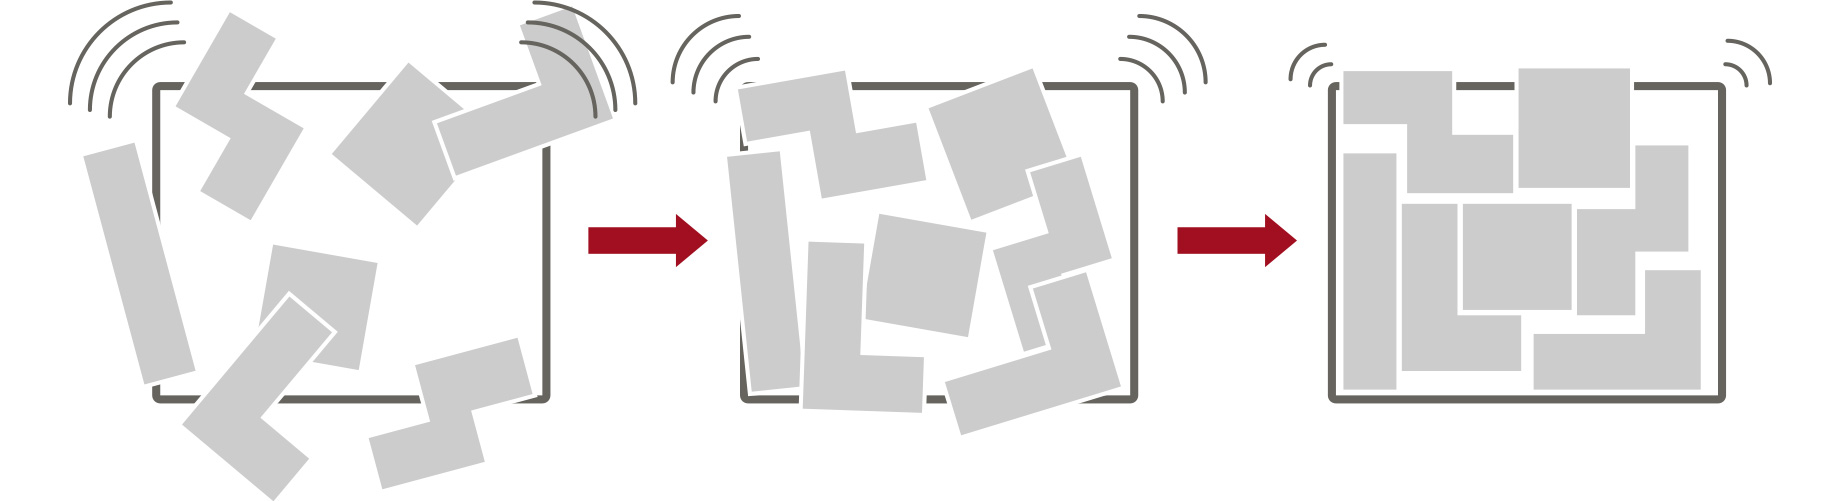
\includegraphics[width=0.58\textwidth]{images/fujitsu.jpg}
  \caption{Fujitsu's Bildhafte Erklärung}
  \label{fig:Annealing}
\end{wrapfigure}
Quantum Annealing ist eine Metaheuristik zum Lösen komplexer Optimierungsprobleme \cite{Feld2019}. Fujitsu -- der Hersteller des Digitalen Annealers, den wir untersuchen --  veranschaulicht Annealing im Allgemeinen anhand eines Puzzles wie in Abbildung \ref{fig:Annealing} zu sehen. Um alle Teile schnell einzupassen, 'schüttelt' man zuerst das ganze System  und reduziert dann das Schütteln kontinuierlich (daher der Name Annealing -- 'Ausglühen'). Es ist also ein Heuristisches Näherungsverfahren bei dem alle Lösungen, einschließlich derjenigen, die weit vom Optimum entfernt sind, erkundet werden um sich sukzessive einer optimalen Lösung anzunähern.\\
Nach Lucas \cite{Lucas2014} lassen sich viele NP-harte Probleme auf eine Energieminimierungsaufgabe abbilden, die als Ising-Modell formuliert sind, und (Quantum) Annealing ist in der Lage, solche Ising-Modell-Probleme in polynomieller Zeit zu lösen  \cite{Kadowaki1998}.\\
Der Digitale Annealer, nachführend auch Fujitsu DAU genannt, bewältigt exakt diese Probleme \cite{Tsukamoto2017}. In der von uns getesteten Version 2 kann er theoretisch vollständig verbundene Ising-Modelle mit 8.192 Bits lösen.\\
Quantum Annealing gehört zum Adiabatischen Quantencomputing, da es auf dem Adiabatischen Theorem der Quantenmechanik basiert: Ein System verbleibt in seinem Eigenzustand, wenn der zeitabhängige Hamiltonoperator sich nur sehr langsam ändert \cite{Griffiths1995}. Der D-Wave Quantencomputer implementiert das Adiabatische Quantencomputing in seiner Hardware und manipuliert die verfügbaren Quantenbit-Zustände (Qubit) gemäß des zeitabhängigen Hamiltonian, nachfolgend als $H(t)$ bezeichnet\cite{Feld2020}.
\begin{equation}
H(t)=s(t) H_{A}+(1-s(t)) H_{P}
\end{equation}
Der Grundgedanke ist die Interpolation zwischen einem Anfangs-Hamiltonian $H_A$, dessen Grundzustand einfach zu konstruieren ist, und einem Problem-Hamiltonian $H_P$, dessen minimale Energiekonfiguration dem globalen Optimum des definierten Problems entspricht \cite{Farhi2000}. Unter Einhaltung des Adiabatischen Theorems fällt $s(t)$ von 1 auf 0  \cite{Feld2020} und liefert mit hoher Wahrscheinlichkeit den Grundzustand von $H_P$\cite{Albash2018}. Dieses Konzept des adiabatischen Quantencomputers, wie ihn D-Wave herstellt, liegt nahe, dass je langsamer eine Annäherung vonstattengeht, desto wahrscheinlicher ist das Resultat ein Optimum. Jedoch sind die Qubits aufgrund der Dekohärenz \cite{Homeister2018} stark mit der Umgebung gekoppelt und werden kontinuierlich beeinflusst. Daher darf der Annealing Prozess nicht zu lange dauern \cite{Marshall2017}. Die benötigte Zeit hängt von der minimalen Energiedifferenz zwischen den beiden niedrigsten Zuständen des interpolierenden Hamiltonians ab \cite{Farhi2000}.
Um Quantum Annealing auf der Hardware von D-Wave zu verwenden, muss das JSSP jedoch zunächst als ein \textit{Quadratic Unconstrained Binary Optimization} Problem formuliert werden. 
%%%%% Zu detailliert ---> Kürzen?
%%%%%%%%%%%%%%%%%%%
%Die  Form dieser QUBO, die der Quantum Annealer minimieren soll, ist:
%\begin{equation}
%\min x^{t} Q x \quad \text { with } x \in\{0,1\}^{n}
%\end{equation}
%wobei $x$ ein Vektor von binären Variablen der Größe $n$ ist und $Q$ eine $n x n$ große reelle Matrix ist, die die Beziehung zwischen den Variablen beschreibt. 
%Angesichts der Matrix $Q$ versucht der Annealing-Prozess, binäre Variablenzuordnungen zu finden, um die Zielfunktion zu minimieren. \cite{Feld2019}
Im D-Wave Advantage sind die Qubits in einem sogenannten Pegasusgraphen (Abbildung \ref{fig:Pegasus}) angeordnet -- mathematisch ein ungerichteter Graph mit Qubits als Knoten und Kopplern als Kanten. In Bezug auf das QUBO-Problem repräsentiert jedes Qubit eine Variable und Koppler zwischen Qubits repräsentieren die Kosten, die mit Qubit-Paaren verbunden sind. Wenn die Problemstruktur nicht direkt in den Pegasusgraphen eingebettet werden kann, können Hilfs-Qubits zu einer sogenannten \textit{Chain} kombiniert werden, um die verfügbaren Kopplungen zu erweitern. \newline

\begin{wrapfigure}{r}{0.3\textwidth}
  \centering
  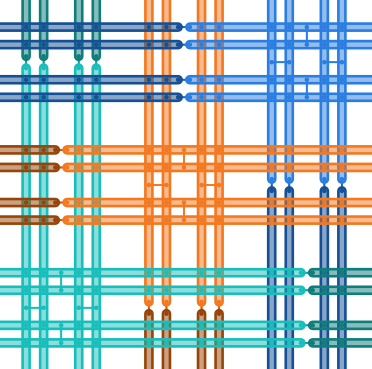
\includegraphics[width=0.28\textwidth]{images/Pegasus.png}
  \caption{Pegasus Topologie mit internen, externen und ungeraden Kopplern}
  \label{fig:Pegasus}
\end{wrapfigure}
Der D-Wave Advantage enthält mindestens 5.000 Qubits mit einer Kopplerdichte von 15 pro Qubit \cite{Advantage2020}. Im Detail besteht die Pegasus-Einheitszelle aus 48 Hälften von Qubits, die zwischen benachbarten  Einheitszellen aufgeteilt sind, wie in Abbildung \ref{fig:Pegasus}: Dabei werden Qubits als abgeschnittene Schleifen (Doppellinien), interne Koppler als Punkte und externe und ungerade Koppler als kurze Linien dargestellt \cite{Pegasus2019}.
Das aktuelle Hauptprobleme besteht darin, dass Quantenhardware hinsichtlich der Anzahl der Qubits und ihrer Konnektivität auf dem Chip begrenzt sind. Da der D-Wave Solver keine All-to-All-Konnektivität implementiert, erschwert es für große QUBO-Probleme ein \textit{minor-embedding} zu finden.
Wenn -- wie bei unserer Problemstellung von TRUMPF -- große Datensätze verwendet werden, kann das resultierende QUBO-Problem die Anzahl der verfügbaren Qubits überschreiten und nicht mehr vollständig auf ein Embedding gebracht werden. Für diesen Fall haben wir noch zwei hybride Lösungsansätze verfolgt, die wir später genauer vorstellen.

\newpage

\subsection{Quantum Gate Model}
\label{subsec:gmodel}
Quantum Gate Modeling (QGM) unterscheidet sich in zweierlei Hinsicht zu klassischen Computern.\\
Zum einen nutzt es das sogenannte „Superpositionsprinzip“, welches einen Qubitzustand als eine Linearkombination aus zwei klassischen Zuständen darstellt. Zum anderen nutzt ein QC das quantenphysikalische Phänomen der „Quantenverschränkung“. Sind zwei quantenphysische Teilchen miteinander verschränkt, so können sie nicht unabhängig voneinander betrachtet werden, sondern werden durch einen gemeinsamen Zustand beschrieben. Diese beiden Konzepte werden in einem sogenannten „Qubit“ vereint.\\ 
Ähnlich wie bei klassischen Bits werden Qubits zu Registern, sog. Quantenregistern zusammengefasst. Ein Quantenregister mit $n$ Qubits repräsentiert dabei die Superposition von $2^{n}$ Zuständen. Genau hier kommt nun das Phänomen der Quantenverschränkung zum Tragen. Einzelne Qubits können miteinander verschränkt werden und liefern damit bei einer Messung des Zustandes kausal verbundene Ergebnisse.\\
Um nun mit den Qubits zu rechnen, gibt es die sogenannten Quantengatter. Diese Gatter ändern mit Hilfe einer physikalischen Aktion, bspw. eines Laserstrahls, die Superposition des Qubits, in dem sie den Spin des Qubits verändern. Daher ist die Dauer der Anwendung von großer Bedeutung. Mathematisch entspricht ein Quantengatter einer unitären Transformation auf ein oder mehrere Qubits, welche als Vektoren dargestellt werden. Damit ist ein Quantengatter eine bijektive unitäre Abbildung und kann mit Hilfe seines adjungierten Operators rückgängig gemacht werden. Dies ist eine Eigenschaft, die klassische Computer nicht erfüllen.\\

Durch diesen Aufbau und diese Funktionsweise kann das Ergebnis eines komplexen Problems in einem Schritt zurückgegeben werden. Ein klassicher Computer bräuchte für ein entsprechendes Ergebnis mehrere Teilschritte.

Das Ergebnis dieser Berechnung wird durch die Superpositionen der einzelnen Qubits erfasst.
Leider können diese Superpositionen nicht direkt physikalisch gemessen werden, denn wird ein Qubit gemessen, so nimmt es einen einzigen Zustand an (entweder $|0\rangle$ oder $|1\rangle$). Durch Wiederholungen dieser Berechnungen und erneutes Messen, kann allerdings die zugrundeliegende Superposition beliebig genau approximiert werden. Auch wenn viele Wiederholungen dabei nötig sind, hat der QC einen erheblichen Geschwindigkeitsvorteil gegenüber klassischen Computern.

\section{Verwandte Arbeiten}
\label{sec:related}
Auch andere Forschungsarbeiten haben verschiedene Typen von Quantenprozessoren miteinander verglichen. Die Hauptmethode dieser Arbeiten besteht darin, denselben Algorithmus auf verschiedenen Prozessoren laufen zu lassen und die Ergebnisse miteinander zu vergleichen.\\
2017 veröffentlichten Forscher an der University of Maryland den Artikel: \textit{'Experimental comparison of two quantum computing architectures'} in dem sie zwei Gattermodell-Architekturen, supraleitende Qubits und Trapped Ion Qubits, vergleichen. Obwohl die beiden Systeme unterschiedliche native Quanteninteraktionen haben, können sie auf eine Weise programmiert werden, die unabhängig für die zugrundeliegende Hardware ist, was einen Vergleich von identischen Quantenalgorithmen auf verschiedenen physikalischen Systemen ermöglicht. Die Forscher haben gezeigt, dass Quantenalgorithmen und -schaltungen, welche eine höhere Konnektivität nutzen, eindeutig von einem besser verbundenen System von Qubits profitieren. Dieses  Experiment zeigt kritische Faktoren der Skalierung von Quantencomputern, wie z.B. die Konnektivität der Qubits und die Expressivität der Gatter. Darüber hinaus deuten die Ergebnisse darauf hin, dass die Abstimmung bestimmter Quantenanwendungen mit der zugrunde liegenden Hardware von entscheidender Bedeutung für den erfolgreichen Einsatz ist\cite{Linke2017}.\\
Des Weiteren haben Forscher des Pharmaunternehmens GlaxoSmithKline (GSK) mit Hilfe von Quantencomputern Experimente durchgeführt und die unterschiedlichen Herangehensweisen von IBM und D-Wave verglichen. Der  Quantum Annealer von D-Wave, kann dabei bereits mit klassischen Computern konkurrieren und einige Probleme lösen. Auf der anderen Seite haben Gate-basierte Quantencomputer, wie der von IBM, noch nicht genügend Qubits, um Probleme von relevanter Komplexität zu lösen. Die GSK-Forscher gehen davon aus, dass die zu erwartende Erhöhung der Qubit-Anzahl in solchen Computern dazu führen wird, dass Quantengeräte einen signifikanten Leistungsvorteil gegenüber klassischer Hardware aufweisen werden\cite{Fox2021}.

\section{Konzept}
\label{sec:concept}
Im folgenden Kapitel werden wir unser grundlegendes Konzept und Vorgehen aufzeigen. Zunächst werden wir auf unsere Constraints und die Kostenfunktion für die QUBO eingehen und die Komplexität des JSSP diskutieren. Anschließend beschreiben wir die angewandten Pruning Methoden, das allgemeine Vorgehen und die eingesetzten Trainingsmethoden.

\subsection{QUBO-Formulierung}
\label{subsec:qubo}
\textit{Quadratic Unconstrained Binary Optimization}, kurz QUBO, ist eine Form zur Beschreibung % NP-harter
kombinatorischer Optimisierungsprobleme.\\
Sie besteht meist aus einer zu minimierenden Kostenfunktion $K$ sowie Straftermen $H_{0}$ bis $H_{n}$, welche dazu dienen, bestimmte Tupelbelegungen zu verbieten. Da ein Quantencomputer nach der Lösung mit dem \textit{niedrigsten} energetischen Level sucht, füllen Strafterme die Matrixfelder, welche diese Belegungen beschreiben, mit \textit{positiven} Energiewerten.\\\\
Wir definieren die QUBO-Variablen  binär:
\begin{equation}
x_{j, p, o, m, t}= \begin{cases}1 & : \adjustbox{stack=ll}{\small{Operation $o$ aus der Order $(j, p)$ wird auf \\ der Maschine $m$ zum Zeitpunkt $t$ gestartet }} \\ 0 & : \text { \small{sonst} }\end{cases}
\end{equation}
Im folgenden sind $O$ – die Menge aller Operationen, $T$ – die Gesamtzeit, die nötig ist, um alle Operationen \textit{nacheinander} auszuführen, $M$ - die Menge aller verfügbaren Maschinen.

Im Folgenden eine Übersicht über unsere Strafterme und Kostenfunktion.
\begin{equation}
H_{0} = \sum_{o\in O} (1 - \sum_{m\in M} \sum_{t=0}^{T-1} x_{j,p,o,m,t})^2
\label{H0}
\end{equation}
Dieser Strafterm stellt sicher, dass für jeden Job jede Operation \textit{genau} einmal gestartet wird. Er bestraft also mehrmalige und fehlende Belegung einer Operation\cite{Denkena2021}.

\begin{align}
&H_{1} = \sum_{j\in J} (\sum_{k, k'\in V_{J}} x_{k}x_{k'})\\
&{V}_{J}= \left\{ \begin{array}{c}
\left((j, p, o, m, t),\left(j^{\prime}, p^{\prime}, o^{\prime}, m^{\prime}, t^{\prime}\right)\right) \in\left(J \times P \times O_{j} \times M \times T\right)^{2} \mid \\
j=j^{\prime} \wedge p=p^{\prime} \wedge\left(c(o)<c\left(o^{\prime}\right)\right) \wedge\left(t^{\prime}<t+d_{o, m}\right)
\end{array} \right\}\\
&Und\, \left.c\right|_{o_{j}}: O_{j} \rightarrow\left\{1, \ldots, n_{j}\right\} \text{\tiny{(=  Reihenfolge der Operationen innerhalb eines Jobs)}}
\label{H1}
\end{align}
Der zweite Strafterm stellt für alle Bauteile aller Jobs sicher, dass die Reihenfolge der Operationstypen untereinander eingehalten wird\cite{Denkena2021}.

\begin{align}
&H_{2} = \sum_{m\in M} (\sum_{k, k'\in W_{m}} x_{k}x_{k'})\\
&\mathrm{W}_{M}=\left\{\begin{array}{c}
\left((j, p, o, m, t),\left(j^{\prime}, p^{\prime}, o^{\prime}, m^{\prime}, t^{\prime}\right)\right) \in(J \times P \times O \times M \times T)^{2} \mid \\
m=m^{\prime} \wedge\left(t \leq t^{\prime}<t+d_{o, m}\right)
\end{array} \right\}
\label{H2}
\end{align}
Dieser letzte Strafterm bewirkt, dass zu jedem Zeitpunkt auf einer Maschine jeweils maximal ein Bauteil bearbeitet wird\cite{Denkena2021}.

\begin{align}
&K = \sum_{j\in J} (1 + sgn(t_{j}^{*} - t{j,deadline}))(t_{j}^{*} - t{j,deadline})\\
&mit\: t_{j}^{*} = \sum_{t=0}^{T}(x_{o^{*},m,t} * d_{o^{*},m})
\label{K}
\end{align}
Zuletzt folgt hier noch die Kostenfunktion, welche die Verspätung der Bauteile des Jobsets in Sekunden zählt und diese dabei für jede weitere Zeiteinheit $(30s)$ die ein spezifisches Bauteil zu spät ist, härter bestraft\cite{Kurowski2020}. Hier repräsentiert $O^{*}$ die letzte Operation $o$ eines Jobs $j$\\
Diese vier Teilgleichungen können nun in der Form:
\begin{equation}
H = \delta K + \alpha H_{0} + \beta H_{1} + \gamma H_{2}
\label{HGesamt}
\end{equation}
zusammengefasst werden und bilden die zu optimierende Funktion $H$ der QUBO.
Die Konstanten $\alpha$ bis $\gamma$ sind die \textit{Gewichtungen}, welche bestimmen wie sehr ein jeweiliger Strafterm die spätere Wahl der Variablen beeinflussen soll.

\begin{figure}[H]
        \centering
        \begin{subfigure}[b]{0.2\textwidth}
            \centering
            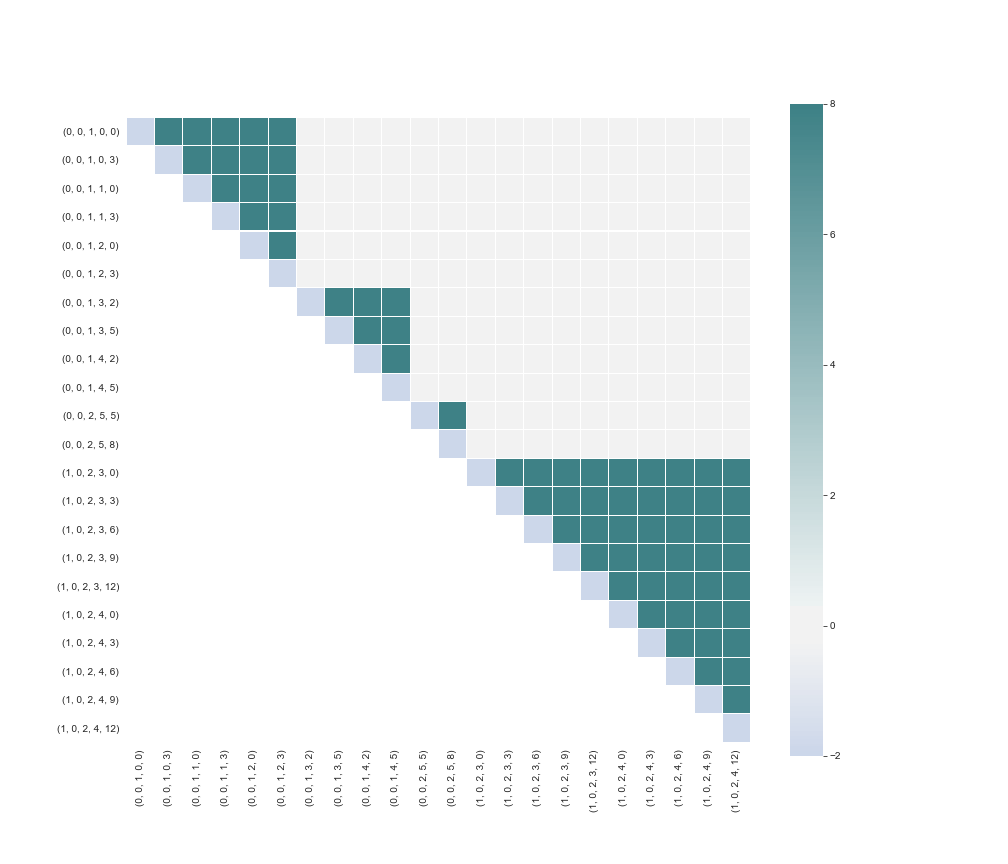
\includegraphics[trim={4.3cm 4.1cm 8.4cm 4.1cm}, clip,width=\textwidth]{images/QUBO_h0.png}
            \caption[]%
            {{\small $H_{0}$}}    
            \label{fig:h0}
        \end{subfigure}
        \hfill
        \begin{subfigure}[b]{0.2\textwidth}
            \centering 
            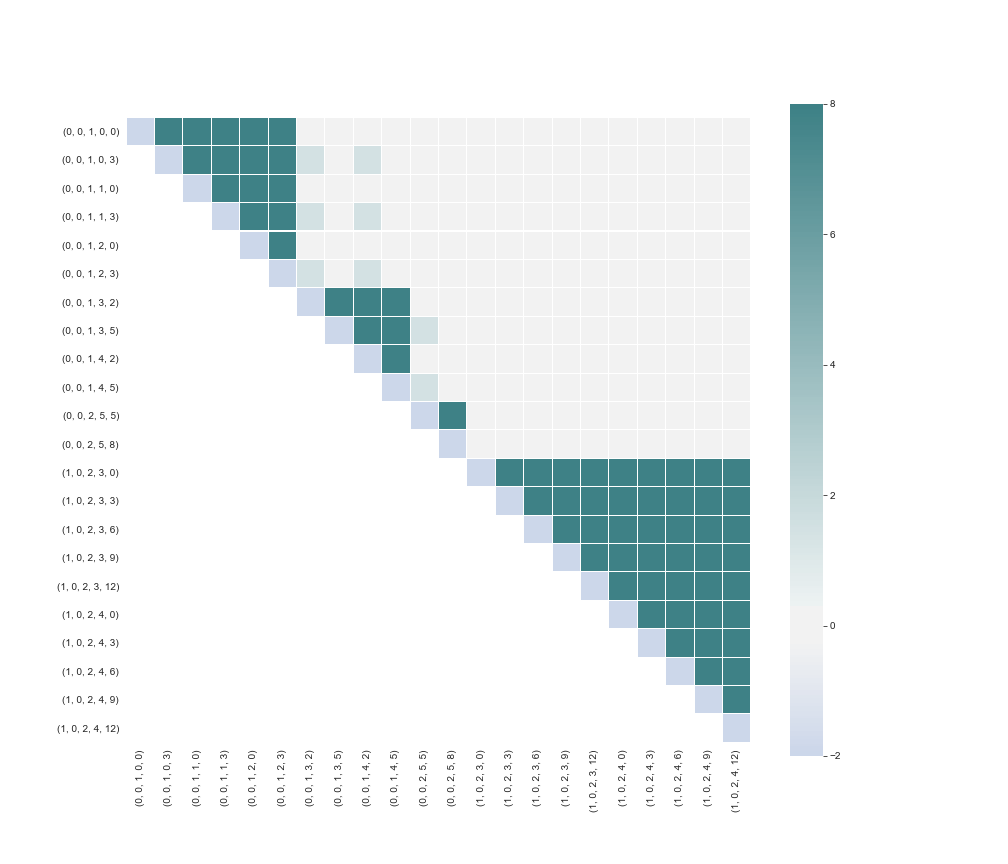
\includegraphics[trim={4.3cm 4.1cm 8.4cm 4.1cm}, clip,width=\textwidth]{images/QUBO_h1.png}
            \caption[]%
            {{\small $H_{1}$}}    
            \label{fig:h1}
        \end{subfigure}
         \hfill
        \begin{subfigure}[b]{0.2\textwidth}
            \centering
            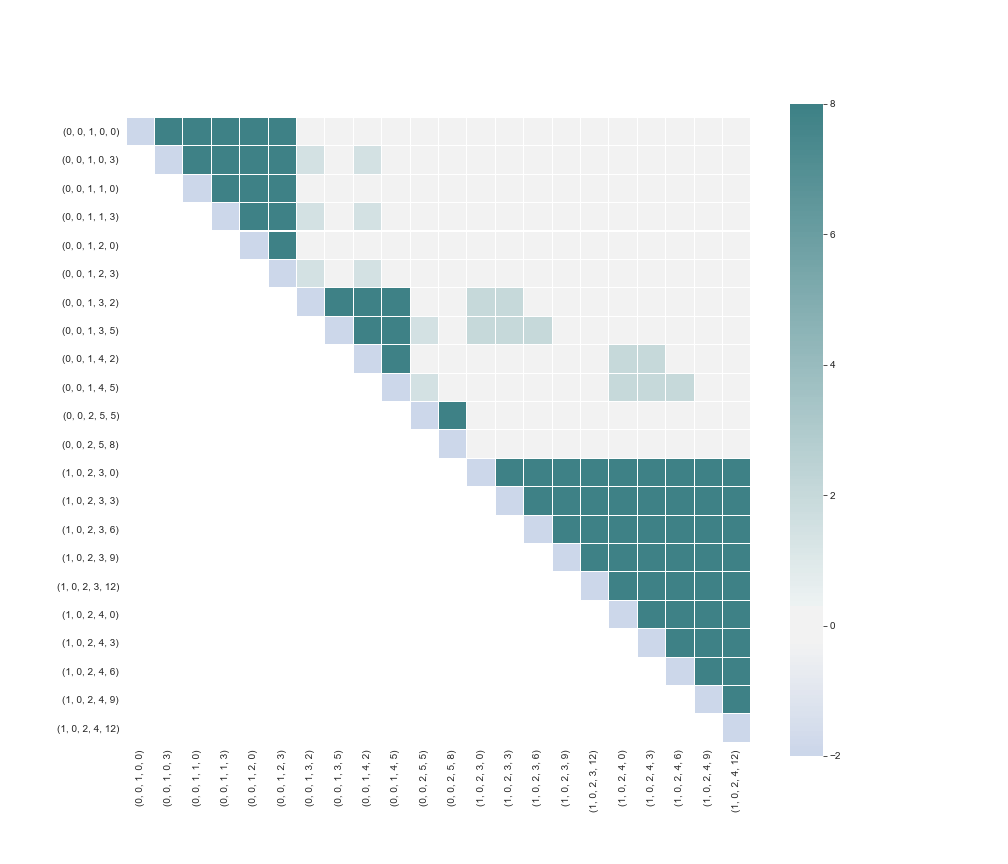
\includegraphics[trim={4.3cm 4.1cm 8.4cm 4.1cm}, clip,width=\textwidth]{images/QUBO_h2.png}
            \caption[]%
            {{\small $H_{2}$}}    
            \label{fig:h2}
        \end{subfigure}
        \hfill
        \begin{subfigure}[b]{0.2\textwidth}
            \centering 
            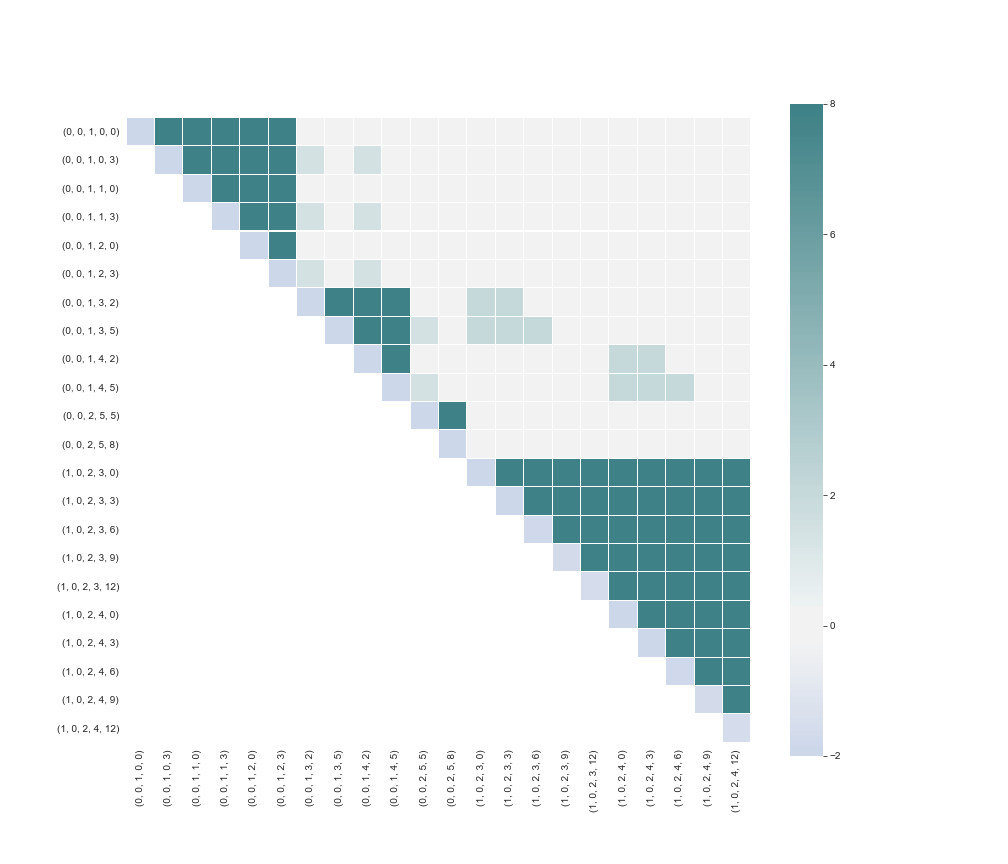
\includegraphics[trim={4.3cm 4.1cm 8.4cm 4.1cm}, clip,width=\textwidth]{images/QUBO_h3.png}
            \caption[]%
            {{\small $K$}}    
            \label{fig:h3}
        \end{subfigure}

        \caption[ Ergebnisse nach Komplexität ]
         {\small Visualisierung des Progressiven Aufbaus der Constraints und Kostenfunktion -- Letztere hat einen merkbar geringeren Effekt vergleichbar zu den Constraints} 
        \label{fig:Results}
    \end{figure}



\subsection{Pruning zur Komplexitätsreduktion}
\label{subsec:pruning}
Eine der wichtigsten Aufgaben während der QUBO-Formulierung war die Eliminierung von möglichst vielen Variablen während des Pruning-Prozesses. Um die Gesamtzahl der Variablen zu reduzieren, haben wir als erstes alle \textit{unmöglichen} Variablen entfernt, deren Index gar nicht existieren kann\cite{Denkena2021}. Zum Beispiel kann eine Biegeoperation nicht auf einer Schweißanlage durchgeführt werden.\\
Zusätzlich haben wir das sogenannte \textit{Heads and Tails} \cite{Venturelli2016} Pruning durchgeführt: für jede Operation muss Zeit für Vorgänger- und Nachfolgeroperationen vorhanden sein. In diesem Schritt haben wir alle Operationen mit unmöglichen Startzeiten entfernt, z. B. Lackieren bei \textit{t} = 0, wenn wir zuvor noch biegen und schweißen müssen. So haben wir alle Variablen $x_{j,p,o,m,t}$ mit $0 \leq t<S$, entfernt, wobei $S$  die Summe der Ausführungszeiten aller Operationen vor der betrachteten ist. Dann haben wir auch alle Variablen $x_{j,p,o,m,t}$ mit  $T-S \leq t <T$ entfernt, wobei $S$ die Summe der Ausführungszeiten aller Operationen nach der betrachteten ist \cite{Kurowski2020}.\\
Den signifikantesten Unterschied machte das \textit{Time-Modulo} Pruning  und hat die Gesamtzahl der Variablen deutlich reduziert. Der Grundgedanke ist es die Gesamtzeiten für jede Operation auf den größten gemeinsamen Teiler zu bringen ohne die Lösungsqualität zu verändern.
Um die Größe unserer QUBO weiter zu reduzieren, haben wir jedoch Zeitstritte von $t_{step} = 30$ Sekunden angenommen. Das ändert nichts für Schweiß- und Lackier-Operationen ($\equiv  \mod  30 sec $), aber addiert in manchen Fällen einen vernachlässigbar kleinen zusätzlichen Zeitpuffer $\Delta t = 10 sec$ am Ende der Biegeoperationen. Dies reduziert die Lösungsqualität geringfügig.

\subsection{Allgemeines Vorgehen}
\label{subsec:approach}
Um eine Vergleichbarkeit unserer Ergebnisse -- die auf verschiedenen Ansätzen und Hardware basieren -- zu erreichen, haben wir einheitliche Problemsets definiert. Diese Problemsets bestehen aus zufällig generierten Job Sets, welche eine gestaffelte Komplexität vorweisen. In Abbildung \ref{fig:JobSets} sind die Gantt-Diagramme mit einer der möglichen optimalen Lösungen (im Nachfolgenden \textit{Best Known Solution -- BKS}) der jeweiligen JSSPs grafisch dargestellt. Die Komplexität dieser Problemsets leitet sich dabei aus der gerundeten Anzahl der Kombinationsmöglichkeiten der verschiedenen Jobs ab.  Die unterschiedlichen Balkenfarben repräsentieren verschiedene Jobs, wobei die Deadline dieser Jobs als kleine Zahl am Balkenende angegeben wurde. (Maschinen, welche nicht genutzt wurden, sind teilweise aus Gründen der Übersichtlichkeit ausgeblendet worden.)
Während das Gate Modeling aufgrund seiner geringen Anzahl an zur Verfügung stehenden Qubits nur Problemsets der Klasse 10 löst, werden beim Annealing die Job Sets 10 bis 500 direkt mit einer QPU und 500 bis 5000 mit Hybriden Ansätzen gelöst. Die QUBO Parameter $\alpha$, $\beta$, $\gamma$ und $\delta$   wurden wie folgt gewählt:
  
\begin{table}[H] \centering 
    \caption{Parameter der QUBO} 
    \label{} 
  \begin{tabular}{@{\extracolsep{4pt}}cccc} 
  \\[-1.8ex]\hline 
  \hline \\[-1.8ex] 
$\alpha$ & $\beta$ & $\gamma$ & $\delta$  \\  
  \hline \\[-1.8ex]
  2.0&1.5&2.0&0.035 \\  
  \hline \\[-1.8ex] 
  \end{tabular} 
  \end{table}
  
Die Constraints sind im Allgemeinen wichtiger als die Kostenfunktion, da diese nicht gebrochen werden dürfen. Sollten sie dennoch gebrochen werden, so wird eine unmögliche Lösung berechnet. Aber auch innerhalb der Constraints gibt es Unterschiede: So führt ein Bruch von $H_0$ ($\alpha$) und $H_2$ ($\gamma$) zu weiteren Seiteneffekten, aber ein Bruch von $H_1$ ($\beta$) lediglich zum Verlust eines einzelnen Bauteils. Daher sind $H_0$ und $H_2$ als \textit{harte} Constraints zu deklarieren, während $H_1$ als ein \textit{weiches} Constraint gilt. Die Kostenfunktion muss anschließend mit Parameter $\delta$ so gewählt werden, dass sie die zuvor definierten Constraints nicht überlagert, jedoch groß genug ist, die optimale Lösung zu finden.
\pagebreak
\newpage

\begin{figure}[H]
        \centering
        \begin{subfigure}[b]{0.445\textwidth}
            \centering
            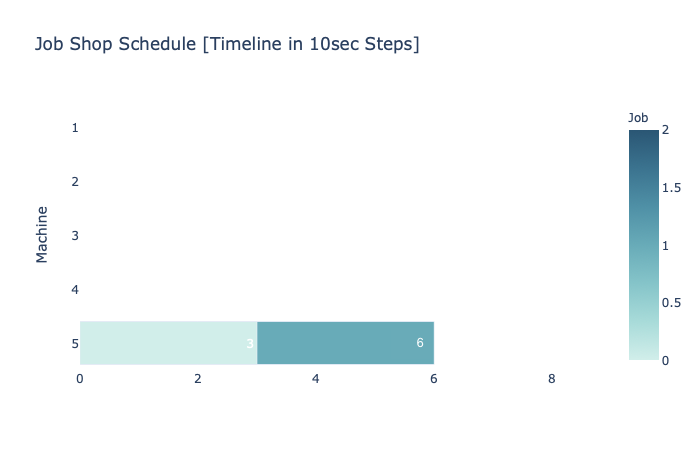
\includegraphics[trim={0 0 2.6cm 0}, clip,width=\textwidth]{images/Job5}
            \caption[]%
            {{\small Job Set 5}}    
            \label{fig:JobSet5}
        \end{subfigure}
        \hfill
        \begin{subfigure}[b]{0.445\textwidth}
            \centering 
            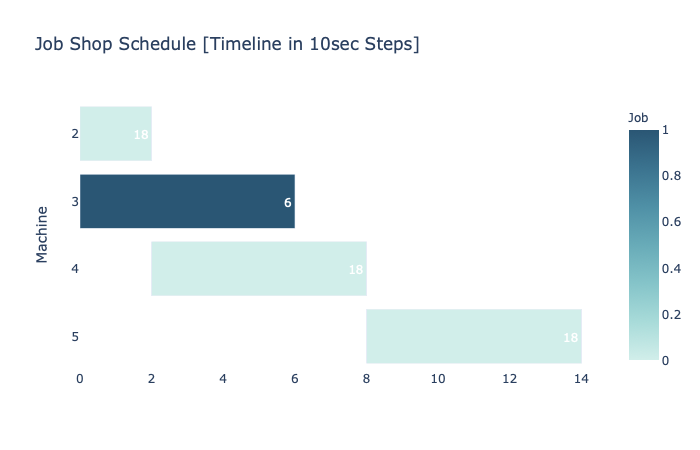
\includegraphics[trim={0 0 2.6cm 0}, clip,width=\textwidth]{images/Job10}
            \caption[]%
            {{\small Job Set 10}}    
            \label{fig:JobSet10}
        \end{subfigure}
        \vskip\baselineskip
        \begin{subfigure}[b]{0.445\textwidth}   
            \centering 
            \includegraphics[trim={0 0 2.6cm 0}, clip, width=\textwidth]{images/Job20}
            \caption[]%
            {{\small Job Set 20}}    
            \label{fig:JobSet20}
        \end{subfigure}
        \hfill
        \begin{subfigure}[b]{0.445\textwidth}   
            \centering 
            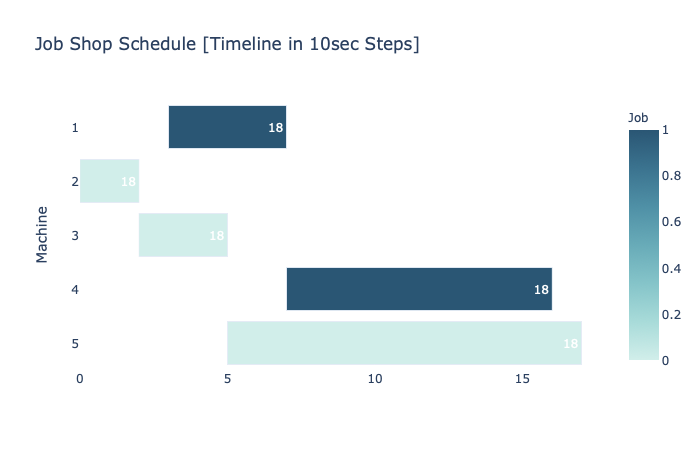
\includegraphics[trim={0 0 2.6cm 0}, clip,width=\textwidth]{images/Job50}
            \caption[]%
            {{\small Job Set 50}}    
            \label{fig:JobSet50}
        \end{subfigure}
        \hfill
        \begin{subfigure}[b]{0.445\textwidth}
            \centering
            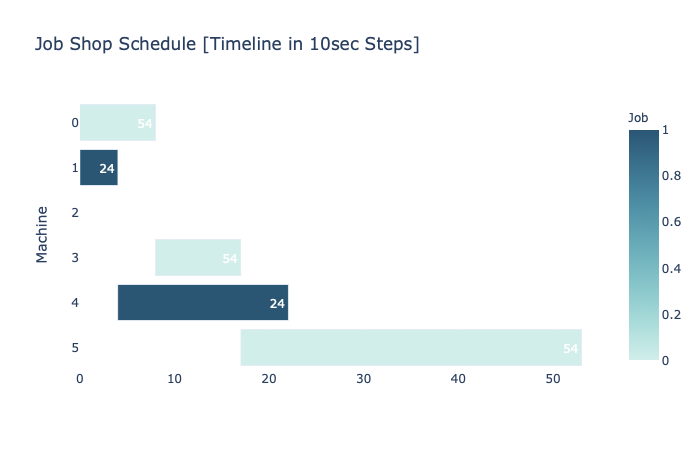
\includegraphics[trim={0 0 2.6cm 0}, clip,width=\textwidth]{images/Job100}
            \caption[]%
            {{\small Job Set 100}}    
            \label{fig:JobSet100}
        \end{subfigure}
        \hfill
        \begin{subfigure}[b]{0.445\textwidth}
            \centering 
            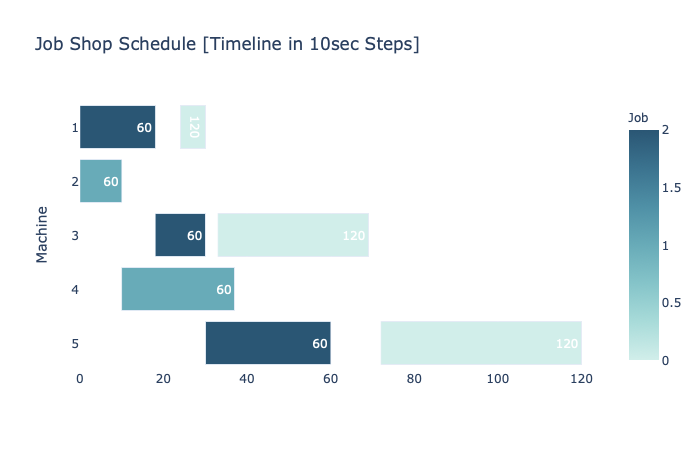
\includegraphics[trim={0 0 2.6cm 0}, clip,width=\textwidth]{images/Job500}
            \caption[]%
            {{\small Job Set 500}}    
            \label{fig:JobSet500}
        \end{subfigure}
        \vskip\baselineskip
        \begin{subfigure}[b]{0.445\textwidth}
            \centering 
            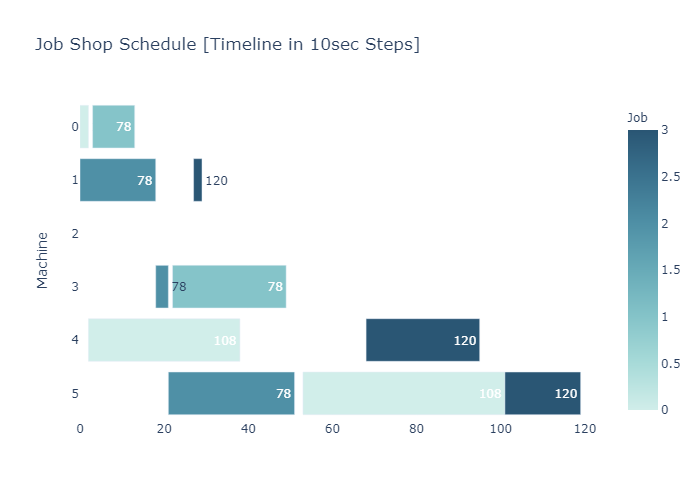
\includegraphics[trim={0 0 2.6cm 0}, clip, width=\textwidth]{images/Job1000}
            \caption[]%
            {{\small Job Set 1000}}    
            \label{fig:JobSet1000}
        \end{subfigure}
        \hfill
        \begin{subfigure}[b]{0.445\textwidth}
            \centering 
            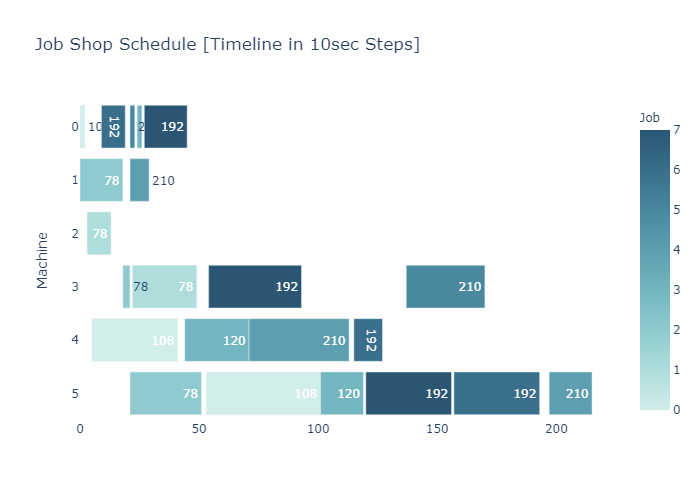
\includegraphics[trim={0 0 2.6cm 0}, clip,width=\textwidth]{images/Job5000}
            \caption[]%
            {{\small Job Set 5000}}    
            \label{fig:JobSet5000}
        \end{subfigure}
        \caption[ Alle Job Sets gestaffelt nach Komplexität ]
         {\small Alle Job Sets gestaffelt nach Komplexität} 
        \label{fig:JobSets}
    \end{figure}

\section{Evaluation}
\label{sec:evaluation}
In diesem Kapitel werden die Ergebnisse der Ansätze des Quantum Annealings und des Quantum Gate Models vorgestellt. Für das Quantum Annealing analysieren wir zunächst die beiden QPUs, deren Parameter und die hybriden Ansätze um größere Probleme zu lösen.
Im Anschluss werden im Gate Model die Ergebnisse von Quantenschaltkreisen vorgestellt.\\
In beiden Teilen werden \textit{Pyschedule} als generischer Solver und \textit{Qbsolv} als klassischer QUBO Solver für Benchmarks genutzt. Für das Annealing werden die beiden Annealer von D-Wave und Fujitsu, der Simulator \textit{Neal} und die hybriden Divide-and-Conquer Ansätze \textit{Leap} und Qbsolv verglichen. Für das Gate Model dienen \textit{Qulacs} und \textit{Qiskit} als Simulatoren und die beiden Quantencomputer von IBM und Rigetti liefern die realen Ergebnisse.  

\subsection{Quantum Annealing}
\label{subsec:annealing}
Im Nachfolgenden werden folgende Solver für die Job-Sets 10 bis 5.000 aus Abbildung \ref{fig:JobSets} miteinander verglichen: \textit{Pyschedule, Qbsolv, D-Wave Neal, Fujitsu DAU, D-Wave Advantage, Qbsolv + D-Wave, D-Wave Leap}.
Als Vergleichswert dient das globale Energieminimum einer \textit{Best Known Solution (BKS)}, also einem Ergebnis, bei dem weder Constraints noch Kostenfunktion verletzt wurden. Des weiteren definieren wir eine  \textit{Good Known Solution (GKS)} als ein Ergebnis bei dem maximal ein Zeitschritt über die Deadline verstrichen ist. Da dies für Alltagssituationen der Lohnfertiger von TRUMPF noch konservativ geschätzt ist, haben wir diesen Maßstab hinzugenommen. Ein Zeitschritt Verspätung entspricht einer Abweichung von 0.5 Energieeinheiten vom Optimum --  also bei D-Wave: $-8.0~\widehat{=}$  BKS und $<-7.5~\widehat{=}$ GKS.

\subsubsection{Ergebnisse}
Unten stehend sind die finalen Ergebnisse der einzelnen Solver nach \textit{BKS} aufgeschlüsselt. Für \textit{Pyschedule} und D-Wave Leap sind keine granularen \textit{BKS}-Werte möglich -- lediglich eine Verifikation.

\begin{table}[!htbp] \centering 
    \caption{Ergebnisse der unterschiedlichen Solver nach Komplexitätsklassen} 
    \label{} 
    \begin{adjustbox}{width=\textwidth}
  \begin{tabular}{@{\extracolsep{4pt}}llcccccccc} 
  \\[-1.8ex]\hline 
  \hline \\[-1.8ex] 
  & & \multicolumn{7}{c}{Komplexitätsklassen der Job-Sets}\\ 
                \cmidrule{3-9}
Type & Solver & Runs& 10 & 20 & 50  & 100& 500&1.000&5.000 \\  
  \hline \\[-1.8ex]
  CPU &Pyschedule &10& \checkmark & \checkmark & \checkmark  & \checkmark& \checkmark&\checkmark&\xmark \\  
  CPU & Qbsolv &10& 100 \%  & 100 \%  & 100 \%   & 62.5 \%\footnotemark  & 100 \%  & 8 \%  & 5 \%   \\  
  CPU &D-Wave Neal &10& 84.2 \%  & 79.2 \%  & 56.2 \%   & 1.6 \%  & 0.6 \%  &0.2 \%  &  \xmark  \\  
  QPU &D-Wave Advantage &20& 26.6 \%  & 1.8 \%   & 0.3 \%   & 0.2 \%  & \xmark &\xmark & \xmark  \\  
  QPU &Fujitsu DAU &15& 99.5 \%  & 31.1 \%   & 4.4 \%   & 1.3 \%  & 0.9 \%  &\xmark &\xmark  \\  
  Hybrid & Qbsolv + D-Wave&1 & 100 \%  & 100 \%   & 100 \%   & 73.2 \%  & 52 \%  &45 \% &100 \%\footnotemark  \\  
  Hybrid& D-Wave Leap&1& \checkmark & \checkmark & \checkmark  & \checkmark& \checkmark&\checkmark&\checkmark \\  
\hline \\[-1.8ex] 
  \end{tabular} 
    \end{adjustbox}
  \end{table}
  
\addtocounter{footnote}{-1}
\footnotetext[2]{In Kapitel \ref{subsubsec:hybrid} werden wir auf diese Anomalie näher eingehen.}
\addtocounter{footnote}{1}
\footnotetext{Aufgrund von mangelnder Rechenzeit nur mit \textit{num\_reads = 1} berechnet.}

Von besonderem Interesse ist der Vergleich der beiden QPUs in Bezug auf Performance und Fehleranfälligkeit. 

\subsubsection{Direkter Vergleich der QPUs}
%Lösungsqualität der QPUs
Im Nachfolgenden haben wir alle QPU Runs nach Komplexität aufgeschlüsselt, um zwei Eigenschaften zu verdeutlichen: Die Solver sind nur für kleine Probleme zuverlässig und die Quantum-Inspired Technologie ist im Streuverhalten dem tatsächlichen Adiabatischen Quantencomputer überlegen. Dies lässt sich auf Quanteneffekte zurückführen, welche jetzt noch zu starken Schwankungen bei den Ergebnissen führen. Außerdem konnte lediglich bis einschließlich Job100 ein Embedding gefunden werden.
\begin{figure}[H]
        \centering
        \begin{subfigure}[b]{0.475\textwidth}
            \centering
            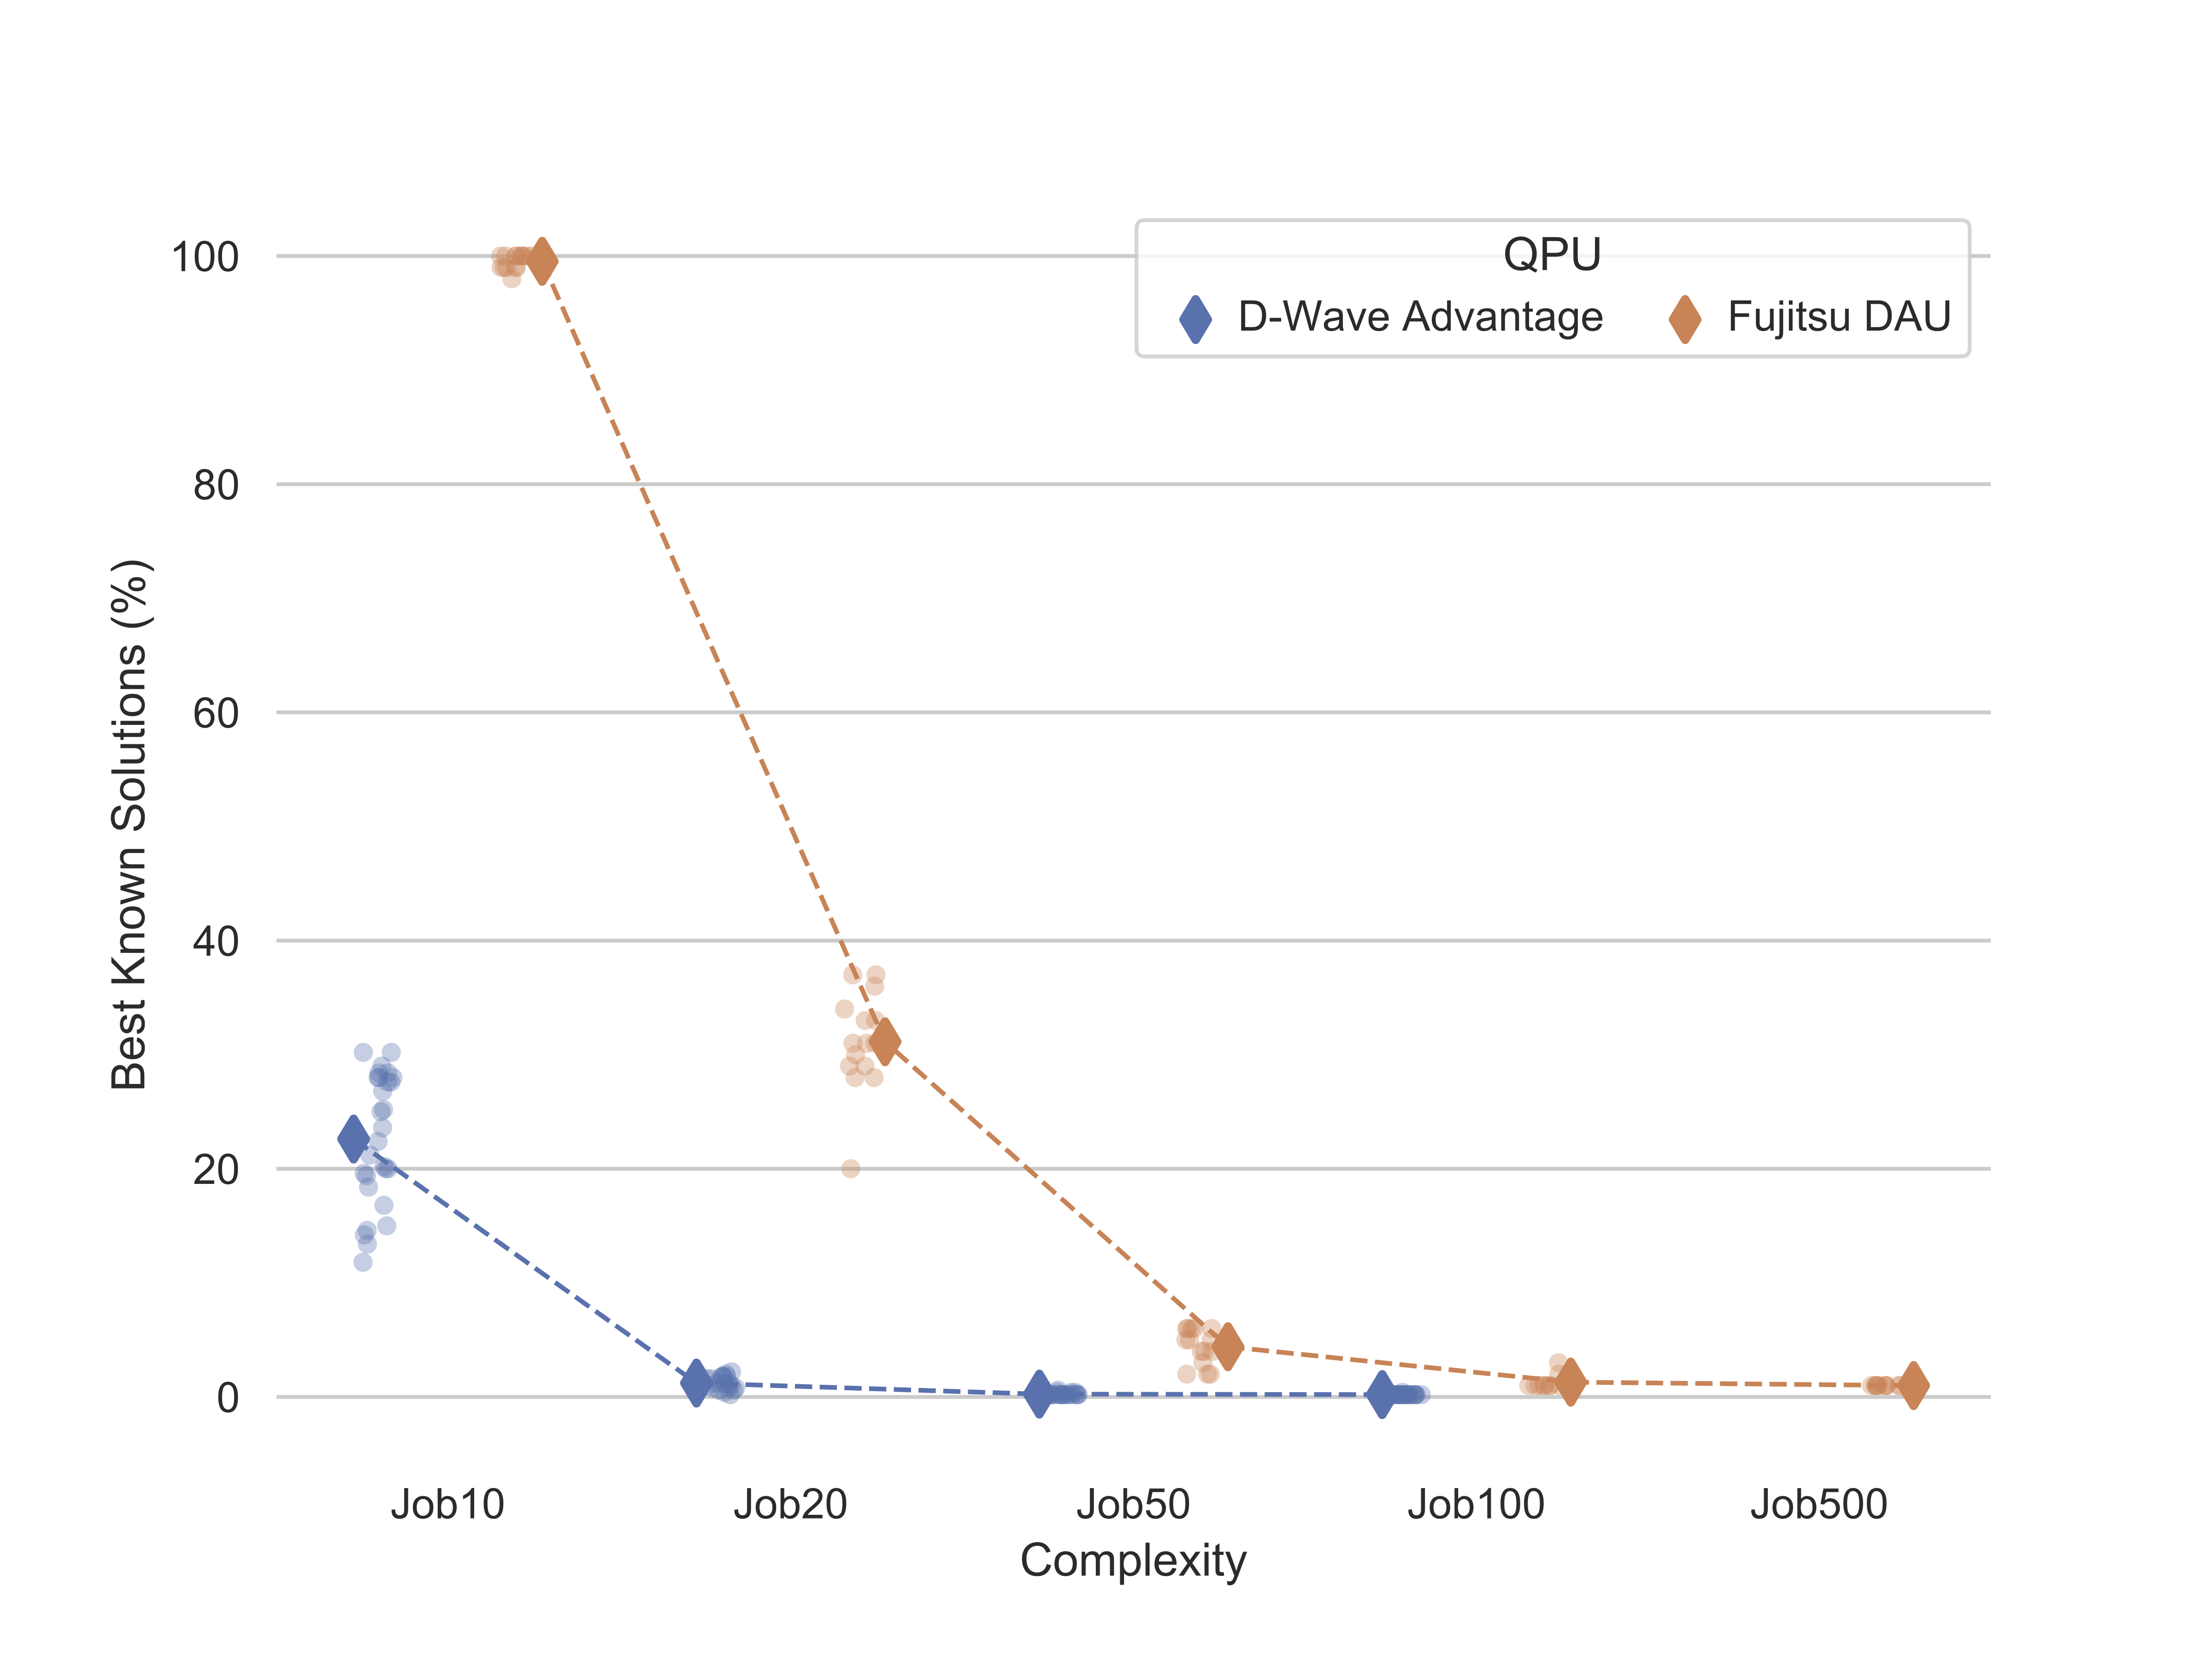
\includegraphics[trim={0.75cm 0.5cm 1.25cm 1.7cm}, clip,width=\textwidth]{images/Best Known Solutions by Complexity.png}
            \caption[]%
            {{\small Best Known Solutions (\%)}}    
            \label{fig:BKS}
        \end{subfigure}
        \hfill
        \begin{subfigure}[b]{0.475\textwidth}  
            \centering 
            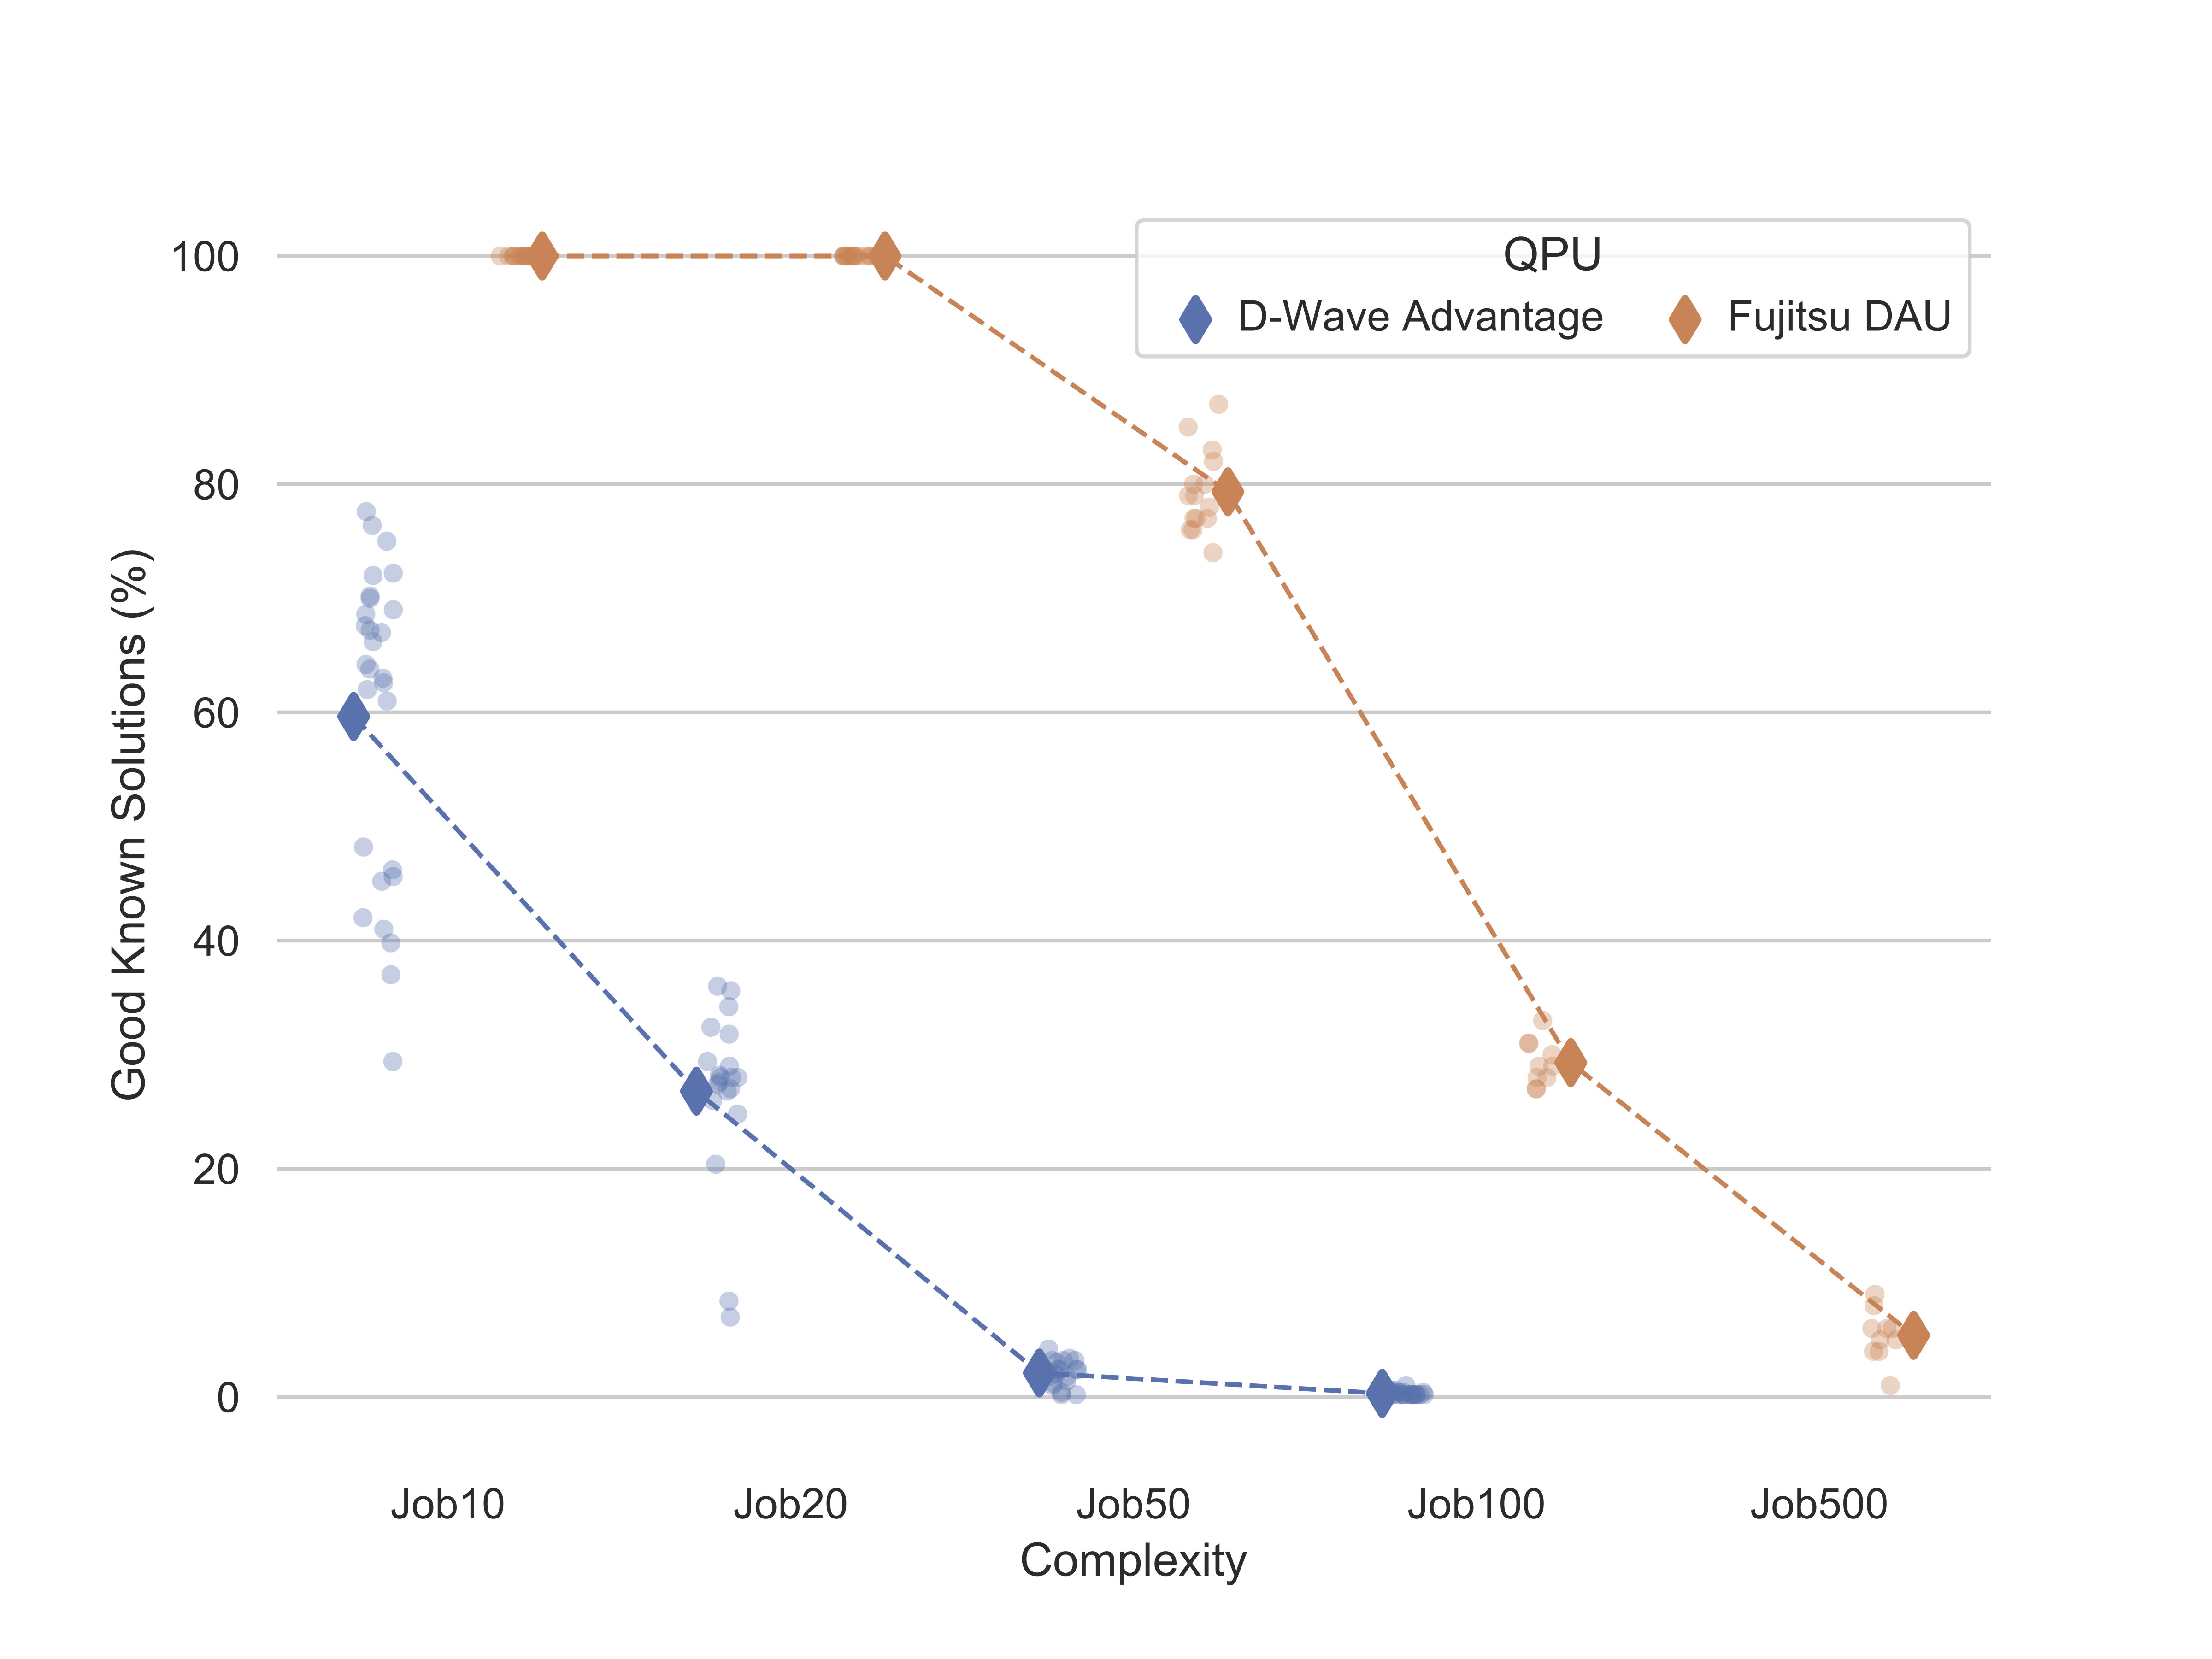
\includegraphics[trim={0.75cm 0.5cm 1.25cm 1.7cm}, clip,width=\textwidth]{images/Good Known Solutions by Complexity.png}
            \caption[]%
            {{\small Good Known Solutions (\%)}}    
            \label{fig:GKS}
        \end{subfigure}
        \caption[ Ergebnisse nach Komplexität ]
         {\small Alle Ergebnisse nach Komplexität} 
        \label{fig:A}
    \end{figure}

Um  dieses Streuverhalten noch genauer zu verdeutlichen, beschränken wir uns nicht nur auf \textit{BKS}  und \textit{GKS},  sondern visualisieren das Gesamtergebnis der Energieminimierung im Ising-Model. Hier erkennt man noch deutlicher, dass bei größeren Komplexitätsklassen der D-Wave Advantage scheinbar zufällige Ergebnisse liefert, während der Fujitsu DAU noch \textit{gute} Lösungen findet.\\

\begin{figure}[H]
        \centering
        \begin{subfigure}[b]{0.495\textwidth}
            \centering
            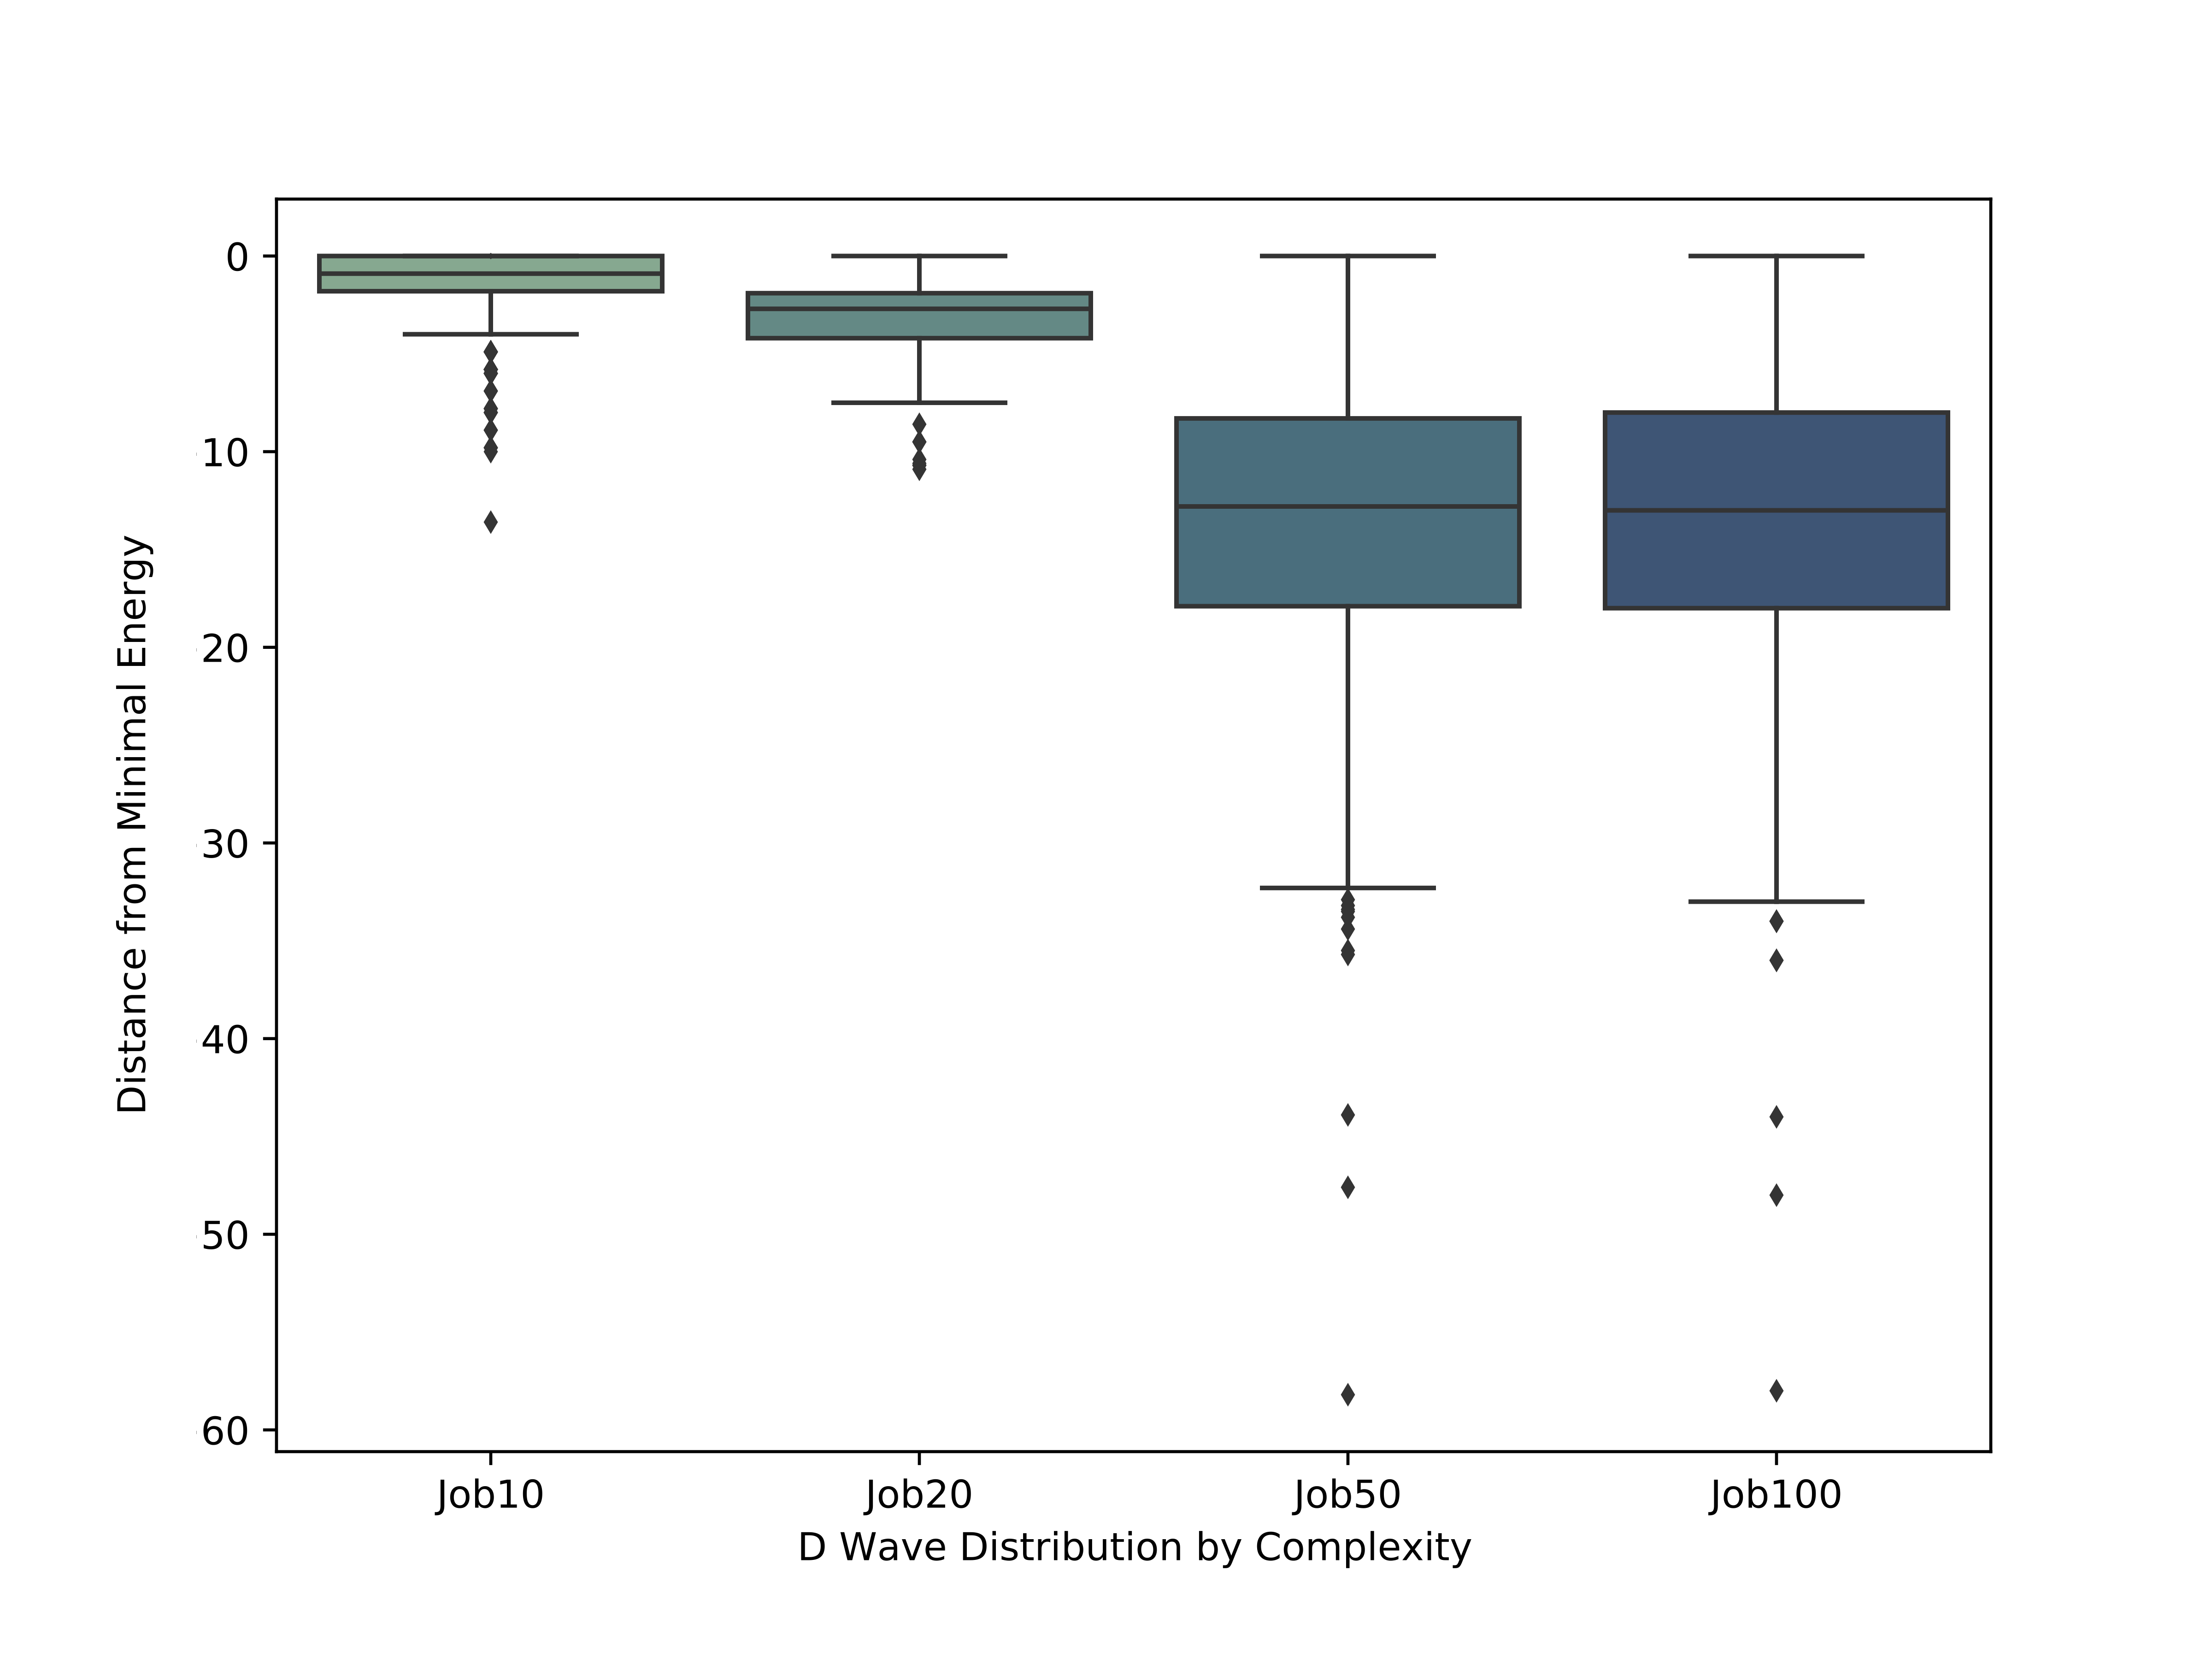
\includegraphics[trim={0 0.7cm 0 1.7cm}, clip,width=\textwidth]{images/D Wave Deviation.png}
            \caption[]%
            {{\small D-Wave Advantage }}    
            \label{fig:DeviationDWave}
        \end{subfigure}
        \hfill
        \begin{subfigure}[b]{0.495\textwidth}  
            \centering 
            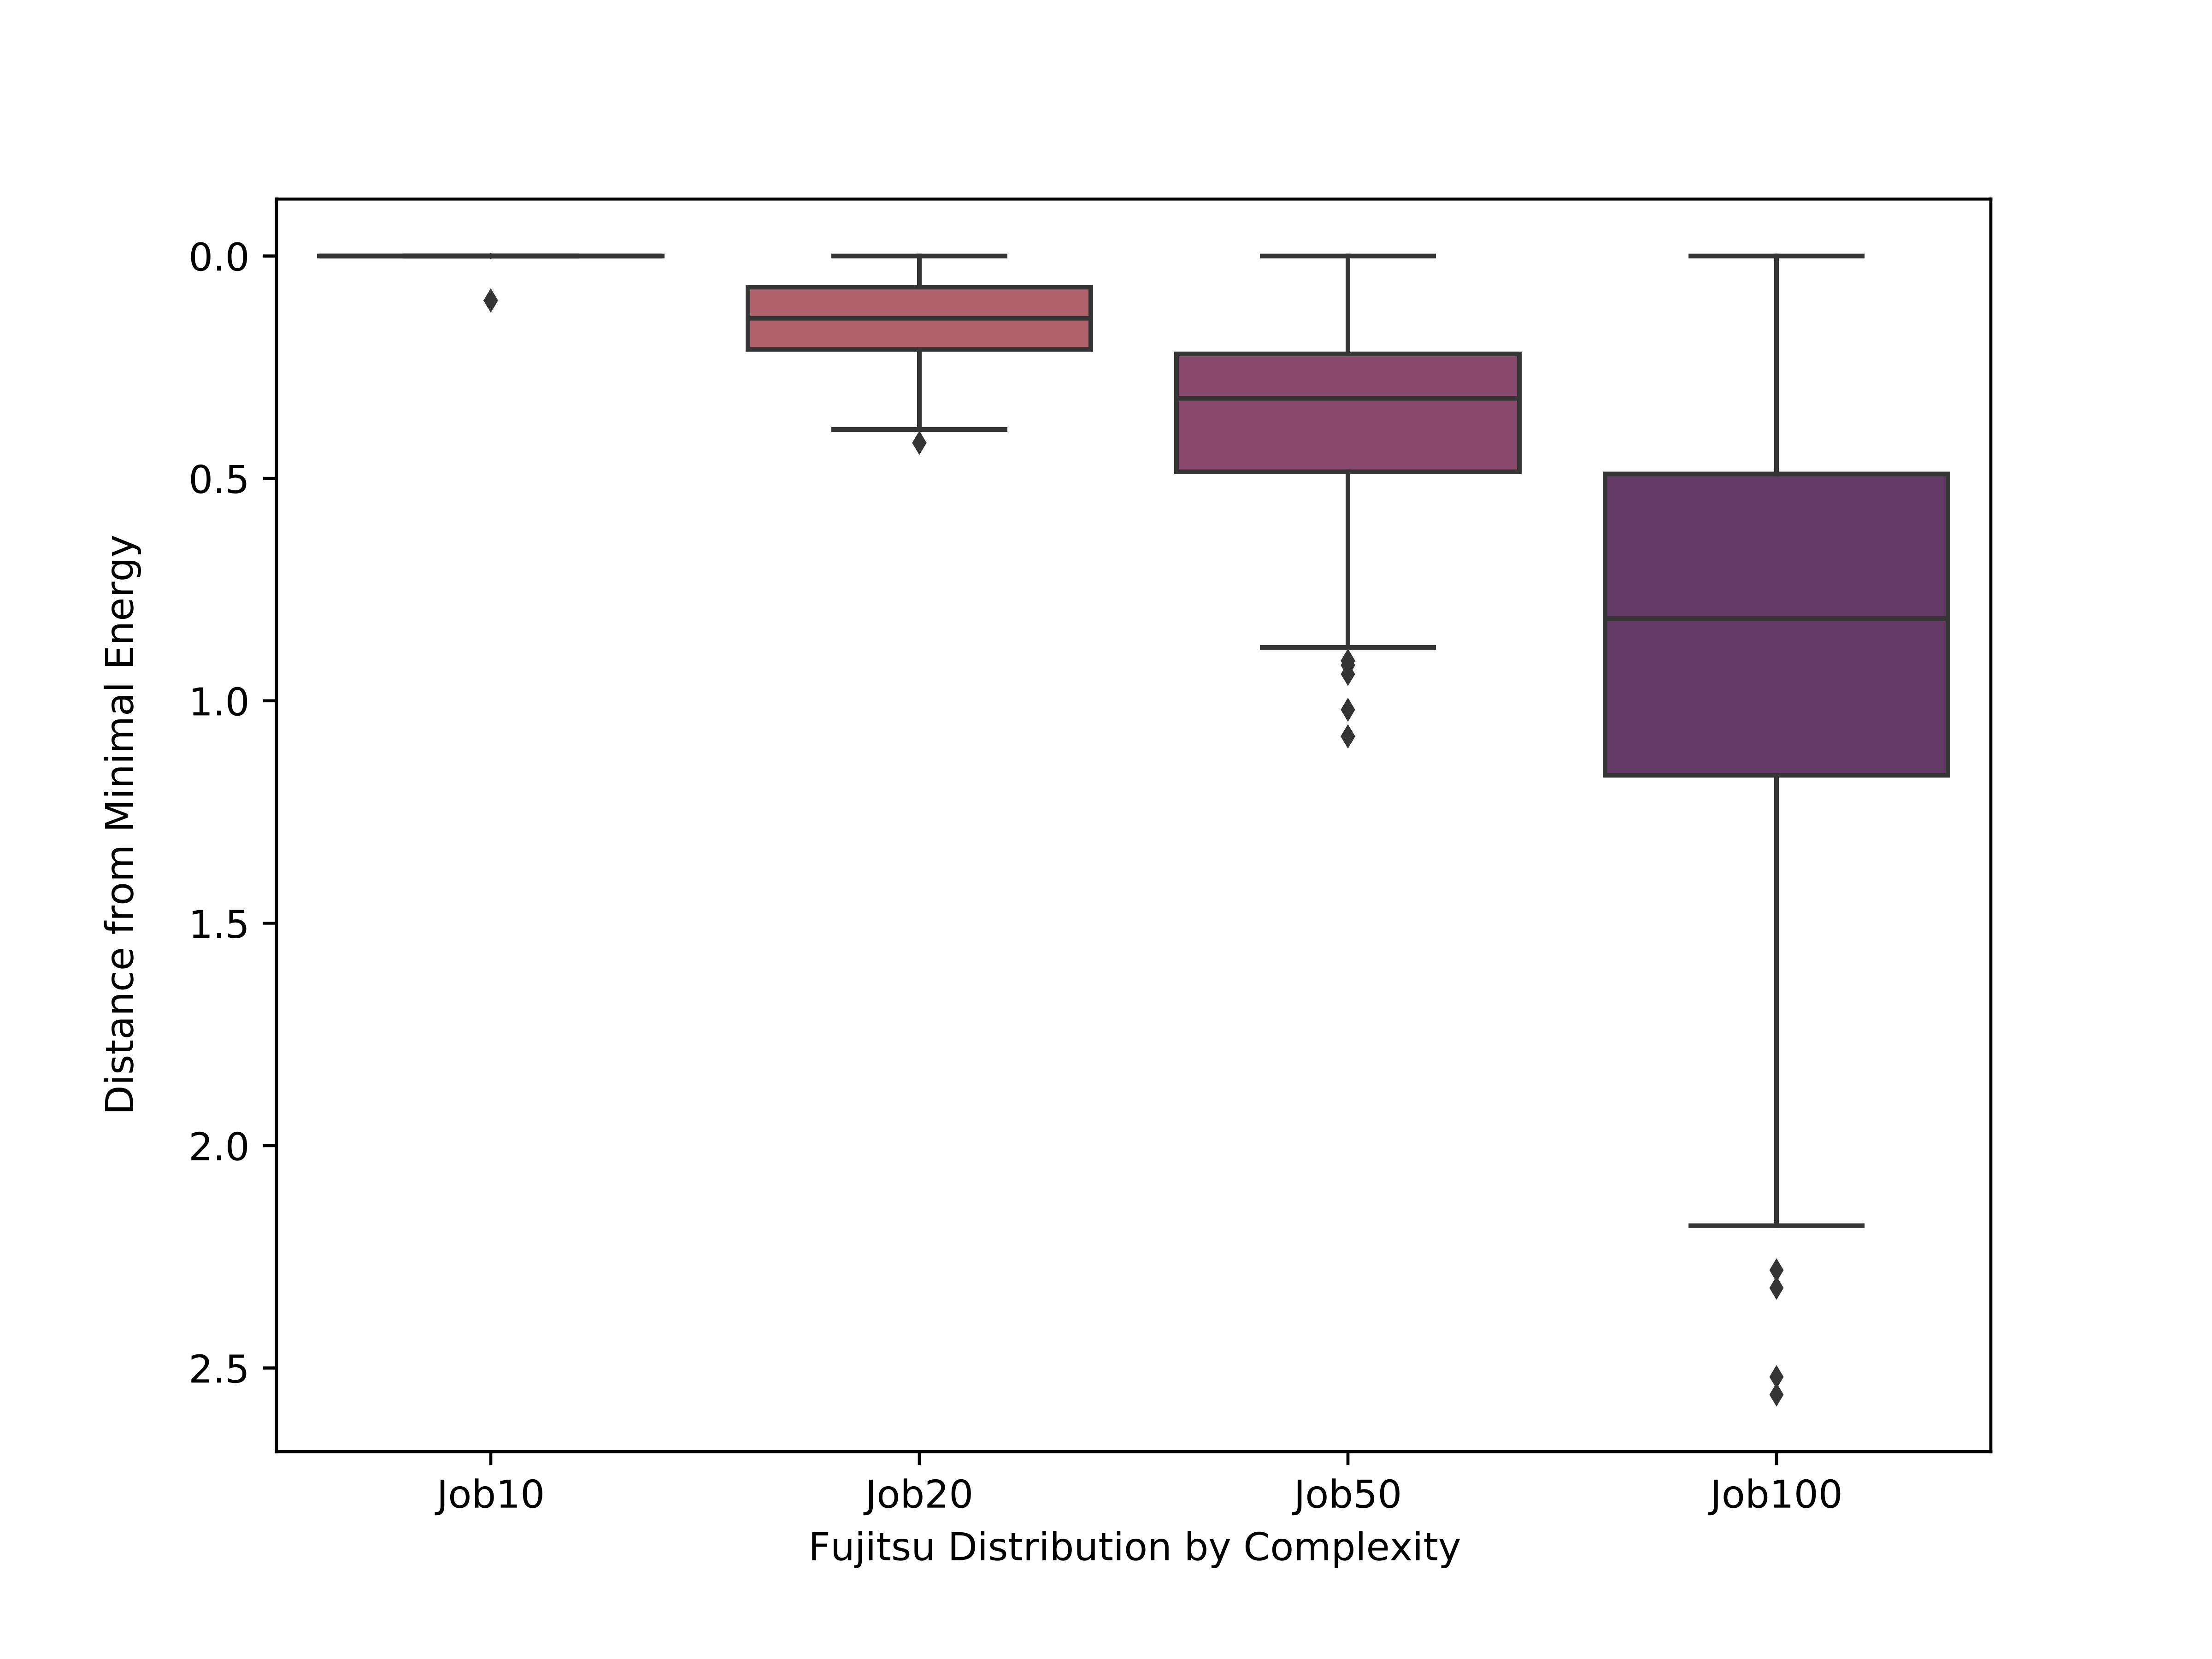
\includegraphics[trim={0 0.7cm 0 1.7cm}, clip,width=\textwidth]{images/Fujitsu Deviation.png}
            \caption[]%
            {{\small Fujitsu DAU}}    
            \label{fig:DeviationFujitsu}
        \end{subfigure}
        \caption[ Ergebnisse nach Komplexität ]
         {\small Alle  Abweichungen vom Energieminimum ($\widehat{=}~0$) nach QPU Solver} 
        \label{fig:Deviation}
    \end{figure}

In Abbildung~\ref{fig:Deviation} erkennt man die starke Streuung genauer. Die Distanz zum Energieminimum (dem globalen Optimum) ist bei allen Ergebnissen des Fujitsu DAU deutlich geringer. Hier bedeutet $0$ das globale Optimum (\textit{BKS}) und $0.5$ entspricht der \textit{GKS}. Die Ergebnisse des D-Wave streuen hingegen bis zu über $50$ Schritte weiter, als die des DAU.
 
\subsubsection{Weitere Parameter des D-Wave Advantage}
Für die  D-Wave Advantage QPU haben wir unseren Lösungsansatz weiter präzisiert um das Maximum an \textit{BKS} zu ermöglichen. 
D-Wave QPUs können Ising-Modelle lösen, aber die erforderliche Konnektivität und Präzision in realen Problemen kann nur erreicht werden, indem die Bits des logischen Modells auf physikalische Qubits abgebildet werden. \cite{QPU2021} Dieser sogenannte Embedding-Prozess reduziert die Anzahl der nutzbaren Modellbits um den Faktor 30-50 im Vergleich zu den verfügbaren Qubits.\cite{Handbook2021} 

Embeddings lassen sich lokal mithilfe  von \textit{minorminer} \cite{Parameter2021} oder remote von D-Wave berechnen und speichern. Dazu haben wir diese verglichen und bewertet nach Gesamt-Performance, Platzierung auf der Pegasus Topologie, Chain-Length, sowie Chain-Breaks. 
Chains entstehen bei der physischen Implementierung eines logischen Qubits mit mehr als einem physischen Qubit. Da diese Konstellation mit zunehmender Distanz (Chain-Length) instabil wird und zu Chain-Breaks führen kann, ist die Chain-Strength als Parameter ausschlaggebend. Als einer der wichtigsten Annealing-Parameter,  stellt sie sicher, dass die physischen Qubits auch den selben Wert abbilden, den die logischen Qubits vorgeben.
Und um diesen Parameter zu bestimmen, haben wir drei Ansätze zur Berechnung verglichen:  Den Maximalwert der QUBO (Empfehlung als Ausgangspunkt von D-Wave), \textit{scale} -- die Skalierung zum größten Problem-Bias und \textit{torque-compensation} -- eine Kompensation für Drehmomente um Chain-Breaks entgegenzuwirken. In Abbildung~\ref{fig:SettingsBKS} kann man anhand der Ergebnisse sehen, dass letzteres am ehesten stetige \textit{BKS} liefert.\\
\begin{wrapfigure}{r}{0.3\textwidth}
  \centering
  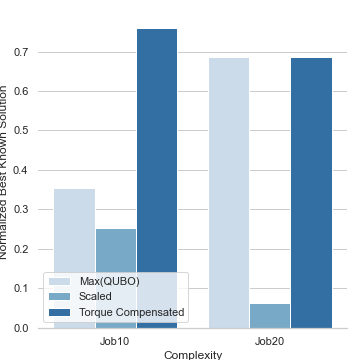
\includegraphics[trim={0.3cm 0.45cm 0.3cm 0.3cm}, clip, width=0.25\textwidth]{images/Chain SettingsBKS}
  \caption{Die Chain Settings für normalisierte BKS von aussagekräftigen Job-Sets}
      \label{fig:SettingsBKS}
      \vspace{-12pt} 
      \end{wrapfigure}
Da sich Quantum Annealing wie in Abschnitt \ref{subsec:anneal} vorgestellt, als zeitliche Balance zwischen Adiabatischem Theorem und der Dekoheränz interpretieren lässt, stellt dies eine weitere Stellschraube in unserer Untersuchung dar.  Die Annealingzeiten haben wir als Fenster um die erwartete optimale Zeit mit wachsender Problemgröße verschoben und analysiert: Die Default Zeit von 20$\mu s$ war meist unter den besten Ergebnissen und andere Einstellungen lieferten kaum Mehrerfolg. Dass die Annealingzeit  mit der Problemgröße steigen muss, hatte nämlich kaum Einfluss: Mit wachsender Komplexität wurden die Ergebnisse insgesamt zunehmend zufällig und damit nicht mehr objektiv vergleichbar unter dem Kriterium Annealingzeit.
Auch die diversen Anneal Schedules (Quench and Pause oder Reverse Annealing), um die Energiewellenform zu ändern, konnten die Lösungsqualität nicht positiv beeinflussen. Nur für die am besten gewählten Parameter (Abbildung \ref{fig:Reverse}) konnten  vergleichbare Ergebnisse von Forward Annealing mit Default Annealing Time erreicht werden.
Zusammenfassend lässt sich sagen, dass sich mit zum Problem passenden Chain Strengths und guten Embeddings die besten Resultate erzielen lassen. Lokal mit  \textit{minorminer} oder remote über D-Wave konnten wir jedoch ab Job500 keine Embeddings mehr berechnen, was für uns die Grenze des D-Wave Advantage als alleinstehenden Solver markiert.

\begin{figure}
        \centering
        \begin{subfigure}[b]{0.875\textwidth}
            \centering
            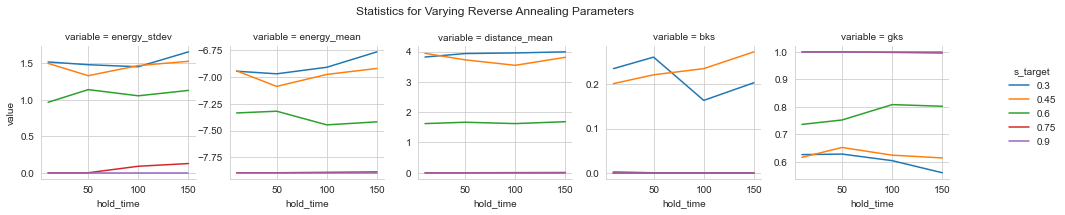
\includegraphics[width=\textwidth]{images/Reverse_s_target}
            \caption[]%
            {{\small Reverse Annealing in Abhängigkeit der Slopes.}}    
            \label{fig:ReverseSlope}
        \end{subfigure}
        \vskip\baselineskip
        \begin{subfigure}[b]{0.875\textwidth}  
            \centering 
            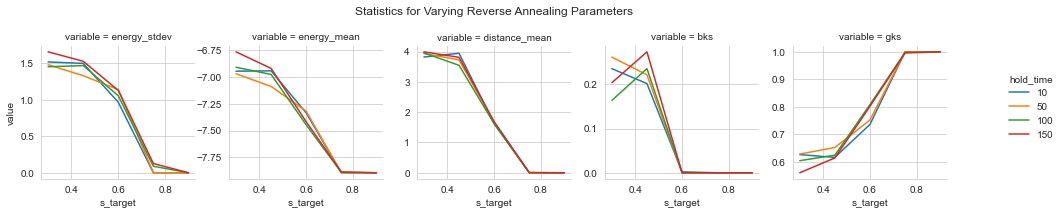
\includegraphics[width=\textwidth]{images/Reverse_hold_time}
            \caption[]%
            {{\small Reverse Annealing in Abhängigkeit der Hold Time.}}    
            \label{fig:ReverseHold}
        \end{subfigure}
        \caption[ Ergebnisse nach Komplexität ]
         {\small Reverse Annealing Parameter mit Random Walk} 
          \label{fig:Reverse}
    \end{figure}


\subsubsection{Hybrider Ansatz mit D-Wave Leap und Qbsolv}
\label{subsubsec:hybrid}
Da wie erwähnt die QPU Solver der aktuellen Generation noch nicht leistungsstark genug sind, um unsere Problemstellungen anzugehen, haben wir uns zusätzlich mit den beiden hybriden Ansätzen auseinandergesetzt: Die Komplettlösung D-Wave Leap \cite{Leap2020} -- eine Kombination aus Decomposer und QPU als Solver -- die aber nur eine finale Lösung zurück gibt und wenig Einblick in die Funktionsweise bietet. Sowie die Kombination aus Qbsolv \cite{Qbsolv2017} als Decomposer, mit dem D-Wave Advantage als QPU. Dieser Ansatz lässt nach jeder Iteration eine Auswertung der Ergebnisse zu. Qbsolv zerlegt dabei die QUBO in kleinere Komponenten (Sub-QUBOs) einer definierten Größe, die dann unabhängig voneinander gelöst werden. Dieser Prozess wird, solange es eine Verbesserung gibt, iterativ ausgeführt. Dabei wird die QUBO-Matrix in jeder Iteration in verschiedene Komponenten aufgeteilt und von der D-Wave QPU gelöst. Neben dem Embedding und Aufspalten der QUBOs in Sub-QUBOs kümmert sich Qbsolv auch um das  Zusammenführen der Lösungen der Teilprobleme. Wir verwenden die Standardkonfiguration von D-Wave's Qbsolv mit $20 \mu s$.\\
Da Qbsolv für Job100 merkbar schlechtere Ergebnisse geliefert hat im Vergleich zu Job50 und Job500 und wir jetzt die Funktionsweise von Qbsolv als Decomposer kennen, kommen wir zu folgender Betrachtung. Da die Sub-QUBO Größe manuell zu bestimmen ist, ist nachfolgender Vergleich interessant: Für zwei Job-Sets -- die sehr ähnlich sind (beide Komplexität 100) und bei direktem QPU Zugriff sehr ähnliche Resultate liefern -- können die Ergebnisse drastisch variieren. Job100 A ist unser zufällig generiertes Problem und Job100 B ein leicht vereinfachtes und manuell konstruiertes Problem.
\begin{figure}[H]
  \centering
  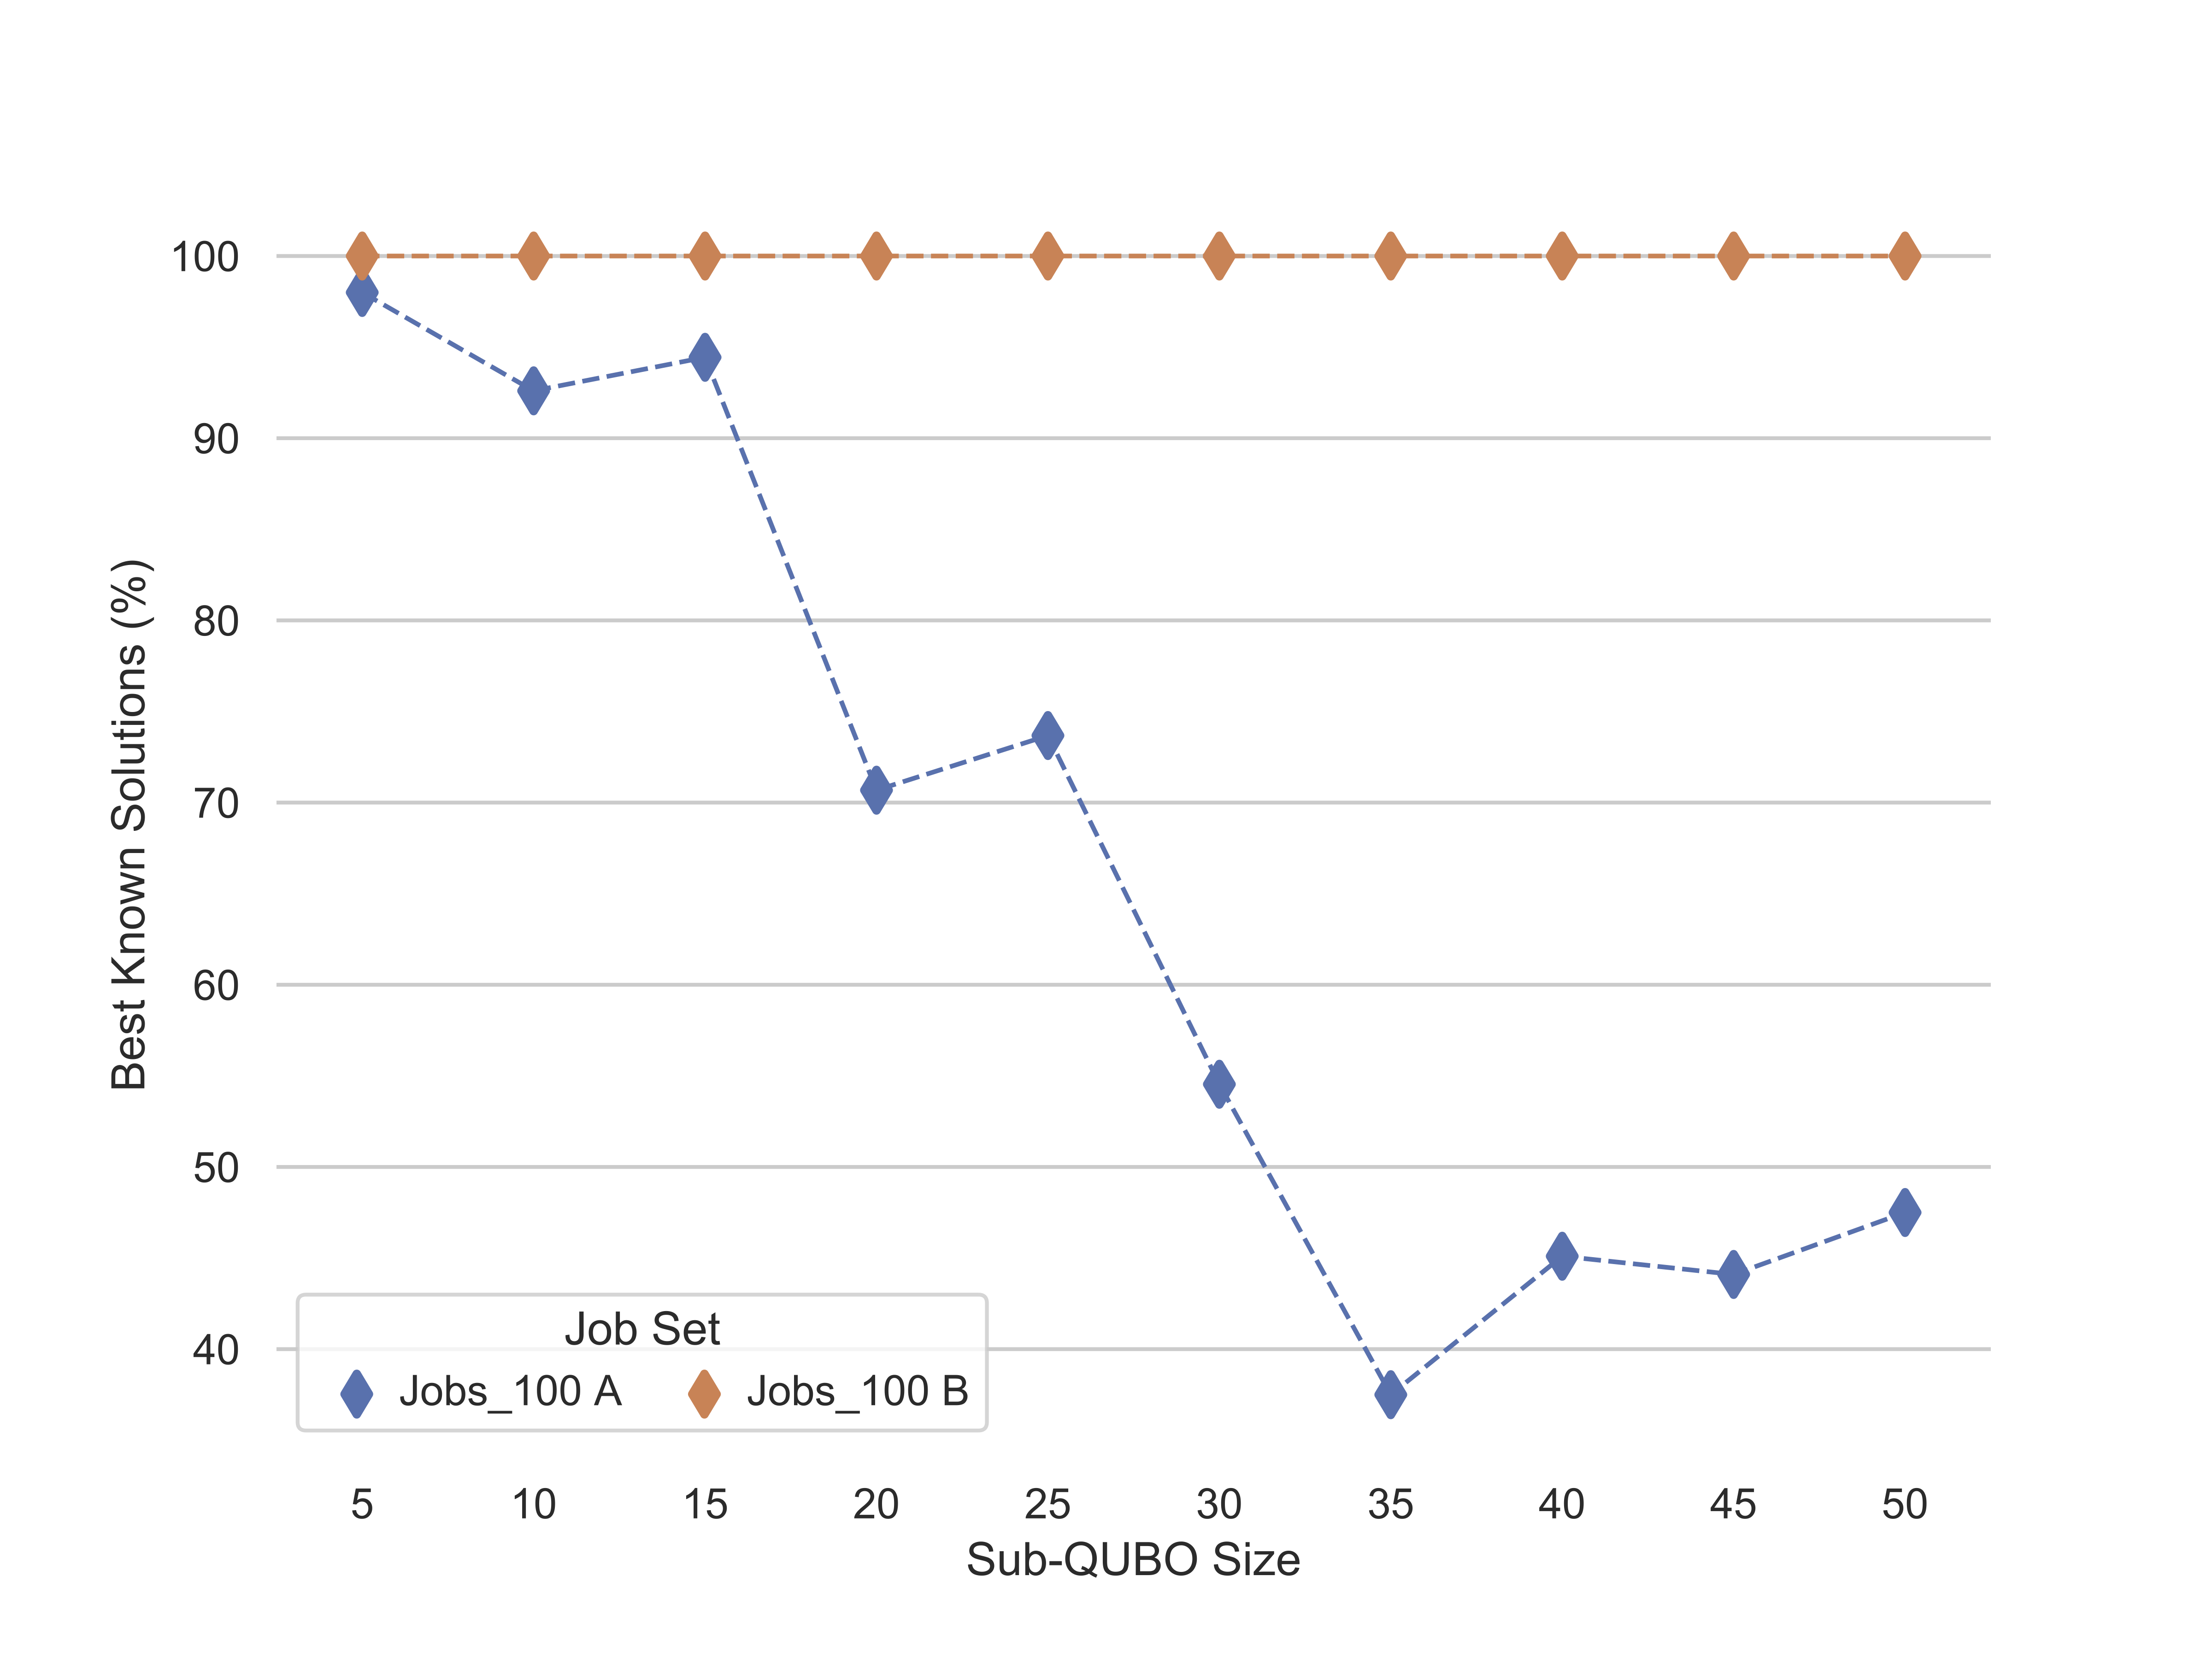
\includegraphics[width=0.45\textwidth]{images/Optimal Sub-QUBO Size.png}
  \label{fig:SubQUBO}
  \caption{BKS (\%) in Abhängigkeit der Sub-QUBO Größe.}
\end{figure}

Während Job100 A mit zunehmender Sub-QUBO Größe deutlich an BKS verliert, kann man bei Job100 B keine Verluste erkennen. Qbsolv als Decomposer schafft es die kleineren Teilprobleme in Job100 B wesentlich effizienter zu strukturieren. Das liegt an einer sehr langen Lackier-Operation in Job100 A, die es erschwert ein Sub-Problem ohne Seiteneffekte zu erstellen.\\\\
Da jedoch alle Teilprobleme  einzeln der Reihe nach remote über D-Wave berechnet werden, erhöht sich die  Gesamtzeit signifikant: Während man $24.7 sec$ reine Rechenzeit für die  $5000 \times 5000$ Matrix  auf der QPU  benötigt, dauerte der hybride Run insgesamt $35 min$. Ein lokaler Vergleich zum Cloud-Service wäre hier interessant. Abschließend zeigt sich aber, dass schon komplexe und größere Probleme mit einem Hybriden Ansatz zu lösen sind. Der Mehrwert der QPU in dieser Konstellation steht jedoch noch aus.

\subsection{Quantum Gate Model}
\label{subsec:qgm}
Im folgenden Teil besprechen und vergleichen wir die Ergebnisse des Quantum Gate Models. Zuerst betrachten wir die Resultate des Qulacs-Simulators, anschließend die Ergebnisse der Quantencomputer \textit{IBM Quantum System One in Ehningen} und des \textit{Rigetti Aspen-9 in Kalifornien}.

Das von uns modellierte Jobset benötigt lediglich vier Qubits. Obwohl uns der IBM Quantum System One 27 Qubits und der Rigetti Aspen-9 32 Qubits zur Verfügungen stellt, stammt die gewählte Komplexität unseres Jobsets aus der Erfahrung, dass mit zunehmender Anzahl der genutzten Qubits die Wahrscheinlichkeit für falsche Ergebnisse durch Quantenrauschen und Dekohärenz ebenfalls enorm wächst.\\
Im folgenden werden die Ergebnisse von Rigetti und IBM durch jeweils zwei Histogramme repräsentiert. Dies liegt an den unterschiedlichen verwendeten Optimierungsansätzen.
Auf der rechten Abbildung wurde der Schaltkreis mit Parametern betrieben, welche zuerst auf einem klassischen Computer voroptimiert und dann zusätzlich auf dem Quantum Computer während der Laufzeit nachoptimiert wurden. Das Diagram auf der linken Seite hingegen gibt die Ergebnisse einer Einspeisung des Schaltkreises mit lediglich klassisch voroptimierten Parametern wieder.

\subsubsection{Qulacs-Simulator}
\begin{wrapfigure}{b!}{0.4\textwidth}
\begin{center}
	\vspace{-15pt}
    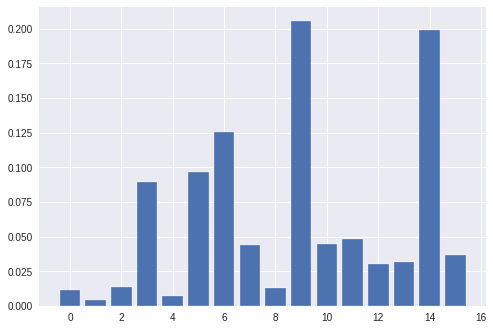
\includegraphics[width=1\linewidth]{images/Qulacs_pre-op_20.png}
  \end{center}
  \caption{Qulacs}
  \vspace{-10pt}
\end{wrapfigure}
Aufgrund der geringen Komplexität der von uns genutzten Jobsets, erlauben es uns klassische Computer noch das Verhalten von Quantencomputern zu simulieren und dabei zuverlässige Ergebnisse zu produzieren.
Wir stützen uns daher bei den folgenden Vergleichen auf die Ergebnisse des Qulacs-Simulators und benutzen diese als Benchmark.
Wie in Abbildung 11 zu sehen ist, stechen zwei Belegungen deutlich hervor. Die größere von beiden, Belegung Nr.9 (Bitstring 1001), repäsentiert hierbei das richtige Ergebnis. Der zweite Ausschlag hingegen gehört zu einer unzulässigen Belegung und ist auf die probabilistische Natur des QCPs zurückzuführen.
    
\subsubsection{IBM Quantum System One}
Die folgenden Ergebnisse stammen von dem neuen Quantencomputer IBM Quantum System One in Ehningen auf den wir im Rahmen dieses Seminars bereits zugreifen konnten.\\
Aus diesem Ergebnis geht hervor, dass der IBMQ ein falsches Ergebnis, Belegung Nr.6 (Bitstring 0110), gewählt hat. Anzumerken ist jedoch, dass das Ergebnis bei dem die Parameter lediglich einfach optimiert wurden (Abbildung \ref{fig:IBM1opt}), wesentlich näher an der korrekten Lösung lagen. Bei einer doppelten Optimierung der Parameter, schneidet die korrekte Belegung deutlich schlechter ab (Abildung \ref{fig:IBM2opt}). Dies könnte darauf hindeuten, dass eine doppelte Optimierung, zumindest auf dem IBM Quantum System One und unter Benutzung des Adam-Optimizers, negative Auswirkungen haben kann.\\
Weiterhin lässt sich beobachten, dass die Varianz der Belegungen bei der einfachen Optimierung (Abbildung \ref{fig:IBM1opt}) deutlich höher ausfällt als bei der doppelten Optimierung (Abbildung \ref{fig:IBM2opt}). Im Allgemeinen kann gesagt werden, dass eine höhere Varianz bei richtigem Ergebnis erstrebenswert ist. Ein einziger großer Ausschlag erhöht hierbei das Vertrauen in die Richtigkeit der berechneten Belegung.

\begin{figure}[H]
        \centering
        \begin{subfigure}{0.49\textwidth}
            \centering
            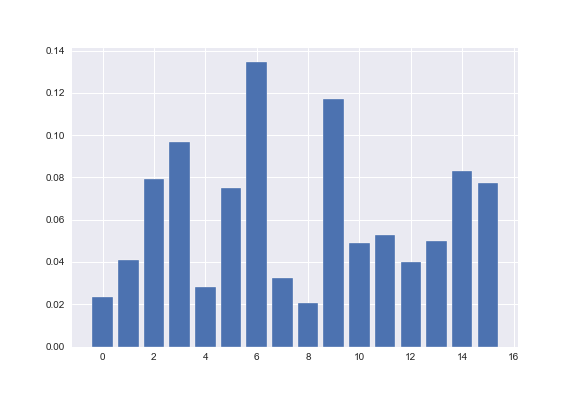
\includegraphics[width=1\linewidth]{images/IBM_small_1opt.png}
            \caption[]%
            {{\small Einfach optimiert}}    
            \label{fig:IBM1opt}
        \end{subfigure}
        \hfill
        \begin{subfigure}{0.49\textwidth}
            \centering 
            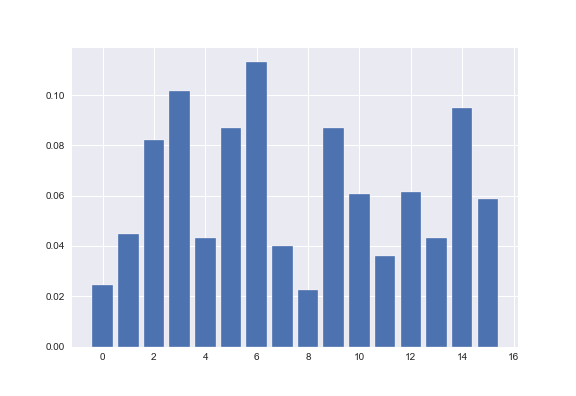
\includegraphics[width=1\linewidth]{images/IBM_small_2opt.png}
            \caption[]%
            {{\small Zweifach optimiert}}    
            \label{fig:IBM2opt}
        \end{subfigure}
        \caption[]%
        {{\small Ergebnisse des IBM Ehningen für ein vier Qubit Jobset}} 
        \label{fig:IBM-Sm-Res}
    \end{figure}

\subsubsection{Rigetti Aspen-9}
Die Ergebnisse des Rigetti Aspen-9 in Kalifornien, angesteuert über AWS Bracket, vervollständigen unseren Vergleich von Quanten-Hardware.\\
Auch hier hat die richtige Belegung nicht den stärksten Ausschlag. Sowohl bei dem einfach optimierten, als auch dem zweifach optimierten Versuch ist die häufigste Belegung die 15 (Bitstring 1111).
Diese Belegung spiegelt die Wahl aller Tupel wieder, was unzulässig ist.\\
Im Gegensatz zu den Ergebnissen des IBM Quantum System One, führt hier die doppelte Parameteroptimierung zu einem besseren Ergebnis. Der Ausschlag der richtigen Belegung ist stärker und die Varianz der Häufigkeiten größer.\\
Das bessere Abschneiden der doppelten Optimierung entspricht viel eher dem erwarteten Unterschied zwischen den beiden Optimierungansätzen.\\\\

Dies hebt die Unterschiede der beiden Quantencomputer nochmals hervor und lässt vermuten, dass die Auffälligkeiten bei unseren IBM Ergebnissen auf die unterschiedlichen Hardwarearchitekturen der beiden Rechner zurückzuführen sind.
Zu guter Letzt stellen wir fest, dass der IBM Quantum System One im Allgemeinen besser auf unseren Schaltkreis anspricht, was die Tatsache, dass er nach der doppelten Optimierung \textit{schlechtere} Ergebnisse zurückgibt, noch bemerkenswerter macht.
 
\begin{figure}[H]
        \centering
        \begin{subfigure}{0.49\textwidth}
            \centering
            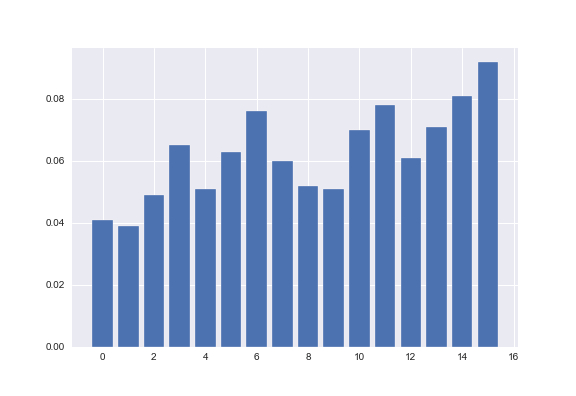
\includegraphics[width=1\linewidth]{images/Rigetti_small_1opt.png}
            \caption[]%
            {{\small Einfach optimiert}}    
            \label{fig:Rig1opt}
        \end{subfigure}
        \hfill
        \begin{subfigure}{0.49\textwidth}
            \centering 
            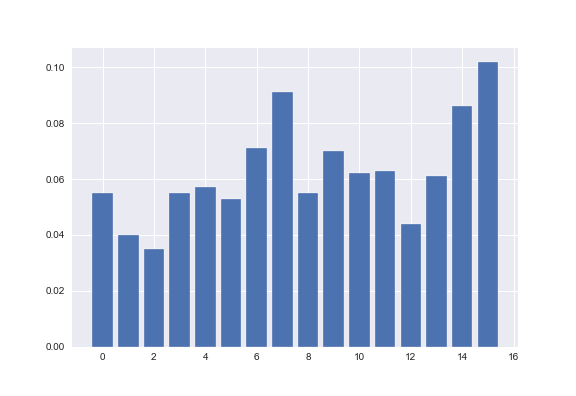
\includegraphics[width=1\linewidth]{images/Rigetti_small_2opt.png}
            \caption[]%
            {{\small Zweifach optimiert}}    
            \label{fig:Rig2opt}
        \end{subfigure}
        \caption[]%
        {{\small Ergebnisse des Rigetti Aspen-9 für ein vier Qubit Jobset}} 
        \label{fig:Rigetti-Sm-Res}
    \end{figure}

\section{Fazit}
\label{sec:conclusion}
In unserem Projekt haben wir die Leistung von mehreren Quantenrechnern anhand eines flexiblen JSSPs für verschiedene Komplexitätklassen verglichen.\\
Unsere Experimente zeigen, dass Quantencomputer in der heutigen NISQ-Ära noch immer keine adäquate Antwort auf das Quantenrauschen haben. Beide Quantum Gate Computer -- IBM Quantum System One und Rigetti Aspen-9 -- konnten keine zufriedenstellenden Lösungen für die gegebenen Jobsets finden.\\
Für kleine Probleminstanzen konnten die Quantum Annealer hingegen schnell qualitativ hochwertige Lösungen finden: beide getesteten QPU Solver waren in der Lage ein JSSP mit bis zu 100 Variablen zu lösen. Dabei war die Quantum-Inspired Technologie von Fujitsu in der Performance und im Streuverhalten dem tatsächlichen Adiabatischen Quantencomputer überlegen. Die besten Ergebnisse lieferten aber hybride Ansätze, mit denen man auch schon jetzt industrienahe Probleme lösen kann.\\
Die QPUs entwickeln sich rasant, so soll die nächste Generation der Digitalen Annealer bis zu einer Millionen binärer Variablen bieten. Bei D-Wave verdoppeln sich alle drei Jahre die Anzahl der verfügbaren Qubits und bei IBM werden in den nächsten Jahren voraussichtlich mehr als ein Tausend Qubits zur Verfügung stehen.\\
All das deutet auf eine vielversprechende Technologie im Kampf gegen exponentiell wachsende Optimierungsprobleme hin.
\newpage

\appendix
\section*{Appendix}

\subsection*{Job Sets nach Komplexität}

\begin{table}[H] \centering 
    \caption{Job5 mit 4 Variablen} 
    \label{} 
  \begin{tabular}{@{\extracolsep{4pt}}cccccc} 
  \\[-1.8ex]\hline 
  \hline \\[-1.8ex] 
OrderNo & PartNo & BendingLines & Weldingpoints & PaintTime & DueDate \\
  \hline \\[-1.8ex]
  0 & 0 & 1 & 0 & 0.5 & 0.5 \\
  1 & 0 & 2 & 0 & 0.5 & 1 \\
  \hline \\[-1.8ex] 
  \end{tabular} 
  \end{table}

\begin{table}[H] \centering 
    \caption{Job10 mit 12 Variablen} 
    \label{} 
  \begin{tabular}{@{\extracolsep{4pt}}cccccc} 
  \\[-1.8ex]\hline 
  \hline \\[-1.8ex] 
OrderNo & PartNo & BendingLines & Weldingpoints & PaintTime & DueDate \\
  \hline \\[-1.8ex]
  0 & 0 & 1 & 2 & 1 & 3 \\
  1 & 0 & 2 & 0 & 0 & 1 \\
  \hline \\[-1.8ex] 
  \end{tabular} 
  \end{table}




\begin{table}[H] \centering 
    \caption{Job20 mit 22 Variablen} 
    \label{} 
  \begin{tabular}{@{\extracolsep{4pt}}cccccc} 
  \\[-1.8ex]\hline 
  \hline \\[-1.8ex] 
OrderNo & PartNo & BendingLines & Weldingpoints & PaintTime & DueDate \\
  \hline \\[-1.8ex]
0 & 0 & 1 & 1 & 2 & 3 \\
  1 & 0 & 0 & 2 & 0 & 1 \\
    \hline \\[-1.8ex] 
  \end{tabular} 
  \end{table}
  

\begin{table}[H] \centering 
    \caption{Job50 mit 49 Variablen} 
    \label{} 
  \begin{tabular}{@{\extracolsep{4pt}}cccccc} 
  \\[-1.8ex]\hline 
  \hline \\[-1.8ex] 
OrderNo & PartNo & BendingLines & Weldingpoints & PaintTime & DueDate \\
  \hline \\[-1.8ex]
0 & 0 & 1 & 1 & 2 & 3 \\
1 & 0 & 2 & 3 & 0 & 3 \\
    \hline \\[-1.8ex] 
  \end{tabular} 
  \end{table}
  
  
\begin{table}[H] \centering 
    \caption{Job100 mit 105 Variablen} 
    \label{} 
  \begin{tabular}{@{\extracolsep{4pt}}cccccc} 
  \\[-1.8ex]\hline 
  \hline \\[-1.8ex] 
OrderNo & PartNo & BendingLines & Weldingpoints & PaintTime & DueDate \\
  \hline \\[-1.8ex]
 0 & 0 & 4 & 3 & 6 & 9 \\
1 & 0 & 2 & 6 & 0 & 4 \\
    \hline \\[-1.8ex] 
  \end{tabular} 
  \end{table}


\begin{table}[H] \centering 
    \caption{Job500 mit 507 Variablen} 
    \label{} 
  \begin{tabular}{@{\extracolsep{4pt}}cccccc} 
  \\[-1.8ex]\hline 
  \hline \\[-1.8ex] 
OrderNo & PartNo & BendingLines & Weldingpoints & PaintTime & DueDate \\
  \hline \\[-1.8ex]
 0 & 0 & 3 & 12 & 8 & 20 \\
 1 & 0 & 5 & 9 & 0 & 10 \\
1 & 1 & 9 & 4 & 5 & 10 \\
    \hline \\[-1.8ex] 
  \end{tabular} 
  \end{table}


\begin{table}[H] \centering 
    \caption{Job1000 mit 1006 Variablen} 
    \label{} 
  \begin{tabular}{@{\extracolsep{4pt}}cccccc} 
  \\[-1.8ex]\hline 
  \hline \\[-1.8ex] 
OrderNo & PartNo & BendingLines & Weldingpoints & PaintTime & DueDate \\
  \hline \\[-1.8ex]
 0 & 0 & 1 & 12 & 8 & 18 \\
 1 & 0 & 5 & 9 & 0 & 13 \\
1 & 1 & 9 & 1 & 5 & 13 \\
 2 & 0 & 1 & 9 & 3 & 20 \\
    \hline \\[-1.8ex] 
  \end{tabular} 
  \end{table}


  
  

\begin{table}[H] \centering 
    \caption{Job5000 mit 5004 Variablen} 
    \label{} 
  \begin{tabular}{@{\extracolsep{4pt}}cccccc} 
  \\[-1.8ex]\hline 
  \hline \\[-1.8ex] 
OrderNo & PartNo & BendingLines & Weldingpoints & PaintTime & DueDate \\
  \hline \\[-1.8ex]
 0 & 0 & 1 & 12 & 8 & 18 \\
 1 & 0 & 5 & 9 & 0 & 13 \\
1 & 1 & 9 & 1 & 5 & 13 \\
 2 & 0 & 1 & 9 & 3 & 20 \\
 3 & 0 & 4 & 14 & 3 & 35 \\
3 & 1 & 1 & 11 & 0 & 35 \\
 4 & 0 & 5 & 4 & 6 & 32 \\
 4 & 1 & 9 & 13 & 6 & 32 \\
    \hline \\[-1.8ex] 
  \end{tabular} 
  \end{table}



\subsection*{Verwendete Einstellungen der Solver}

\begin{table}[H] \centering 
    \caption{Unsere Default Annealing Einstellung bei Fujitsu} 
    \label{} 
  \begin{tabular}{@{\extracolsep{4pt}}p{2.5cm}p{3cm}p{6cm}} 
  \\[-1.8ex]\hline 
  \hline \\[-1.8ex] 
Parameter & Wert & Bedeutung \\ 
 \hline \\[-1.8ex]
solver & DAU & Digital Annealer Unit \\
 solution mode & COMPLETE & Gibt von jedem Durchlauf die beste Lösung an \\
 number runs & 100 & Gesamtanzahl der Durchläufe \\
 number iterations & 500 &  Gesamtanzahl der Iterationen pro Durchlauf \\
temperature start & $1000.0$ & Starttemperatur \\
 temperature end & 1.0 & Endtemperatur \\
  temperature interval & 100 & Anzahl Iterationen (Temperatur konst.) \\
temperature mode & 0 & Temperatur wird pro temperature-interval um den Faktor \textit{1-temperature-decay} verringert \\
 offset increase rate & $0.0$ & Dynamische Energiefunktion  \\
 optimization method & annealing & Unterstützte Optimierungsmethode \\
 annealer version & 2 & Digital Annealer Version \\
 auto tuning & 0 & Automatisches Tuning des QUBOs \\
 bit precision & 16 & Bit-Präzision (In DAU Version 2) \\
    \hline \\[-1.8ex] 
  \end{tabular} 
  \end{table}
  


\begin{table}[H] \centering 
    \caption{Unsere Default Annealing Einstellung bei D-Wave Advantage} 
    \label{} 
  \begin{tabular}{@{\extracolsep{4pt}}p{2.5cm}p{3cm}p{6cm}} 
  \\[-1.8ex]\hline 
  \hline \\[-1.8ex] 
Parameter & Wert & Bedeutung \\ 
 \hline \\[-1.8ex]
 solver & DWave Advantage & Solver mit  5000 Qubits \\
 sampler & Embedding Composite  & D-Waves Sampler für  automatisches Minor-embedding\\
  sampler &  FixedEmbedding Composite & D-Waves Sampler für fixes Minor-embedding\\
 num reads & 500 & Gesamtanzahl der Durchläufe \\
annealing time & $20 \mu s$ & Zeit in Mikrosekunden für ein Annealing (Durchlauf)  \\ 
 \hline \\[-1.8ex] 
  \end{tabular} 
  \end{table}
  

  
  
  \begin{table}[H] \centering 
    \caption{Unsere Default Einstellung bei Hybrid: Qbsolv + D-Wave } 
    \label{} 
  \begin{tabular}{@{\extracolsep{4pt}}p{2.5cm}p{3cm}p{6cm}} 
  \\[-1.8ex]\hline 
  \hline \\[-1.8ex] 
Parameter & Wert & Bedeutung \\ 
 \hline \\[-1.8ex]
 solver & D-Wave Advantage  & Solver mit 5000 Qubits \\
 solver &   D-Wave Neal &   Quantum Annealing Simulator \\
 num reads & 20 & Gesamtanzahl der Durchläufe \\
solver limit & 20 & Maximale Größe der subQUBO Matrix  \\
 \hline \\[-1.8ex] 
  \end{tabular} 
  \end{table}


\subsection*{Berechnungsgrundlagen}

Formeln zur Berechnungsgrundlage für die Chain Strength mit:
\begin{itemize}
\item QUBO $Q=\left(c_{i j}\right)$, 
\item $n$:  Anzahl von $c_{i j} \neq 0$ in $Q$, 
\item mit $i>j$,
\item und  $\langle d\rangle$: Durchschnitt der Verbindungen von Variablen in der QUBO 

\end{itemize}
\vspace{5mm}

\textbf{MaxQUBO:}
\vspace{5mm}
 \begin{equation}
 \max \left(\operatorname{abs}\left(c_{i j}\right)\right)+1
 \end{equation}
\vspace{10mm}

\textbf{Scaled\footnote{Scaled gibt $1$ zurück, falls kein \textit{Binary Quadratic Model} erkannt wird.}:}
\vspace{5mm}
 \begin{equation}
 \max \left(\max \left(\max _{i>i} c_{i j},-\min _{i>i} c_{i j}\right), \max \left(\max _{i=i} c_{i j},-\min _{i=j} c_{i j}\right)\right)
 \end{equation}
\vspace{10mm}

\textbf{Uniform Torque Compensation:}
\vspace{5mm}
 \begin{equation}
 \sqrt{\langle d\rangle * \frac{2 \sum_{i>j} c_{i j}^{2}}{n}}
 \end{equation}
\vspace{15mm}



\subsection*{Weitere Auswertungen}
 \begin{figure}[H]
        \centering
        \begin{subfigure}[b]{0.495\textwidth}
            \centering
            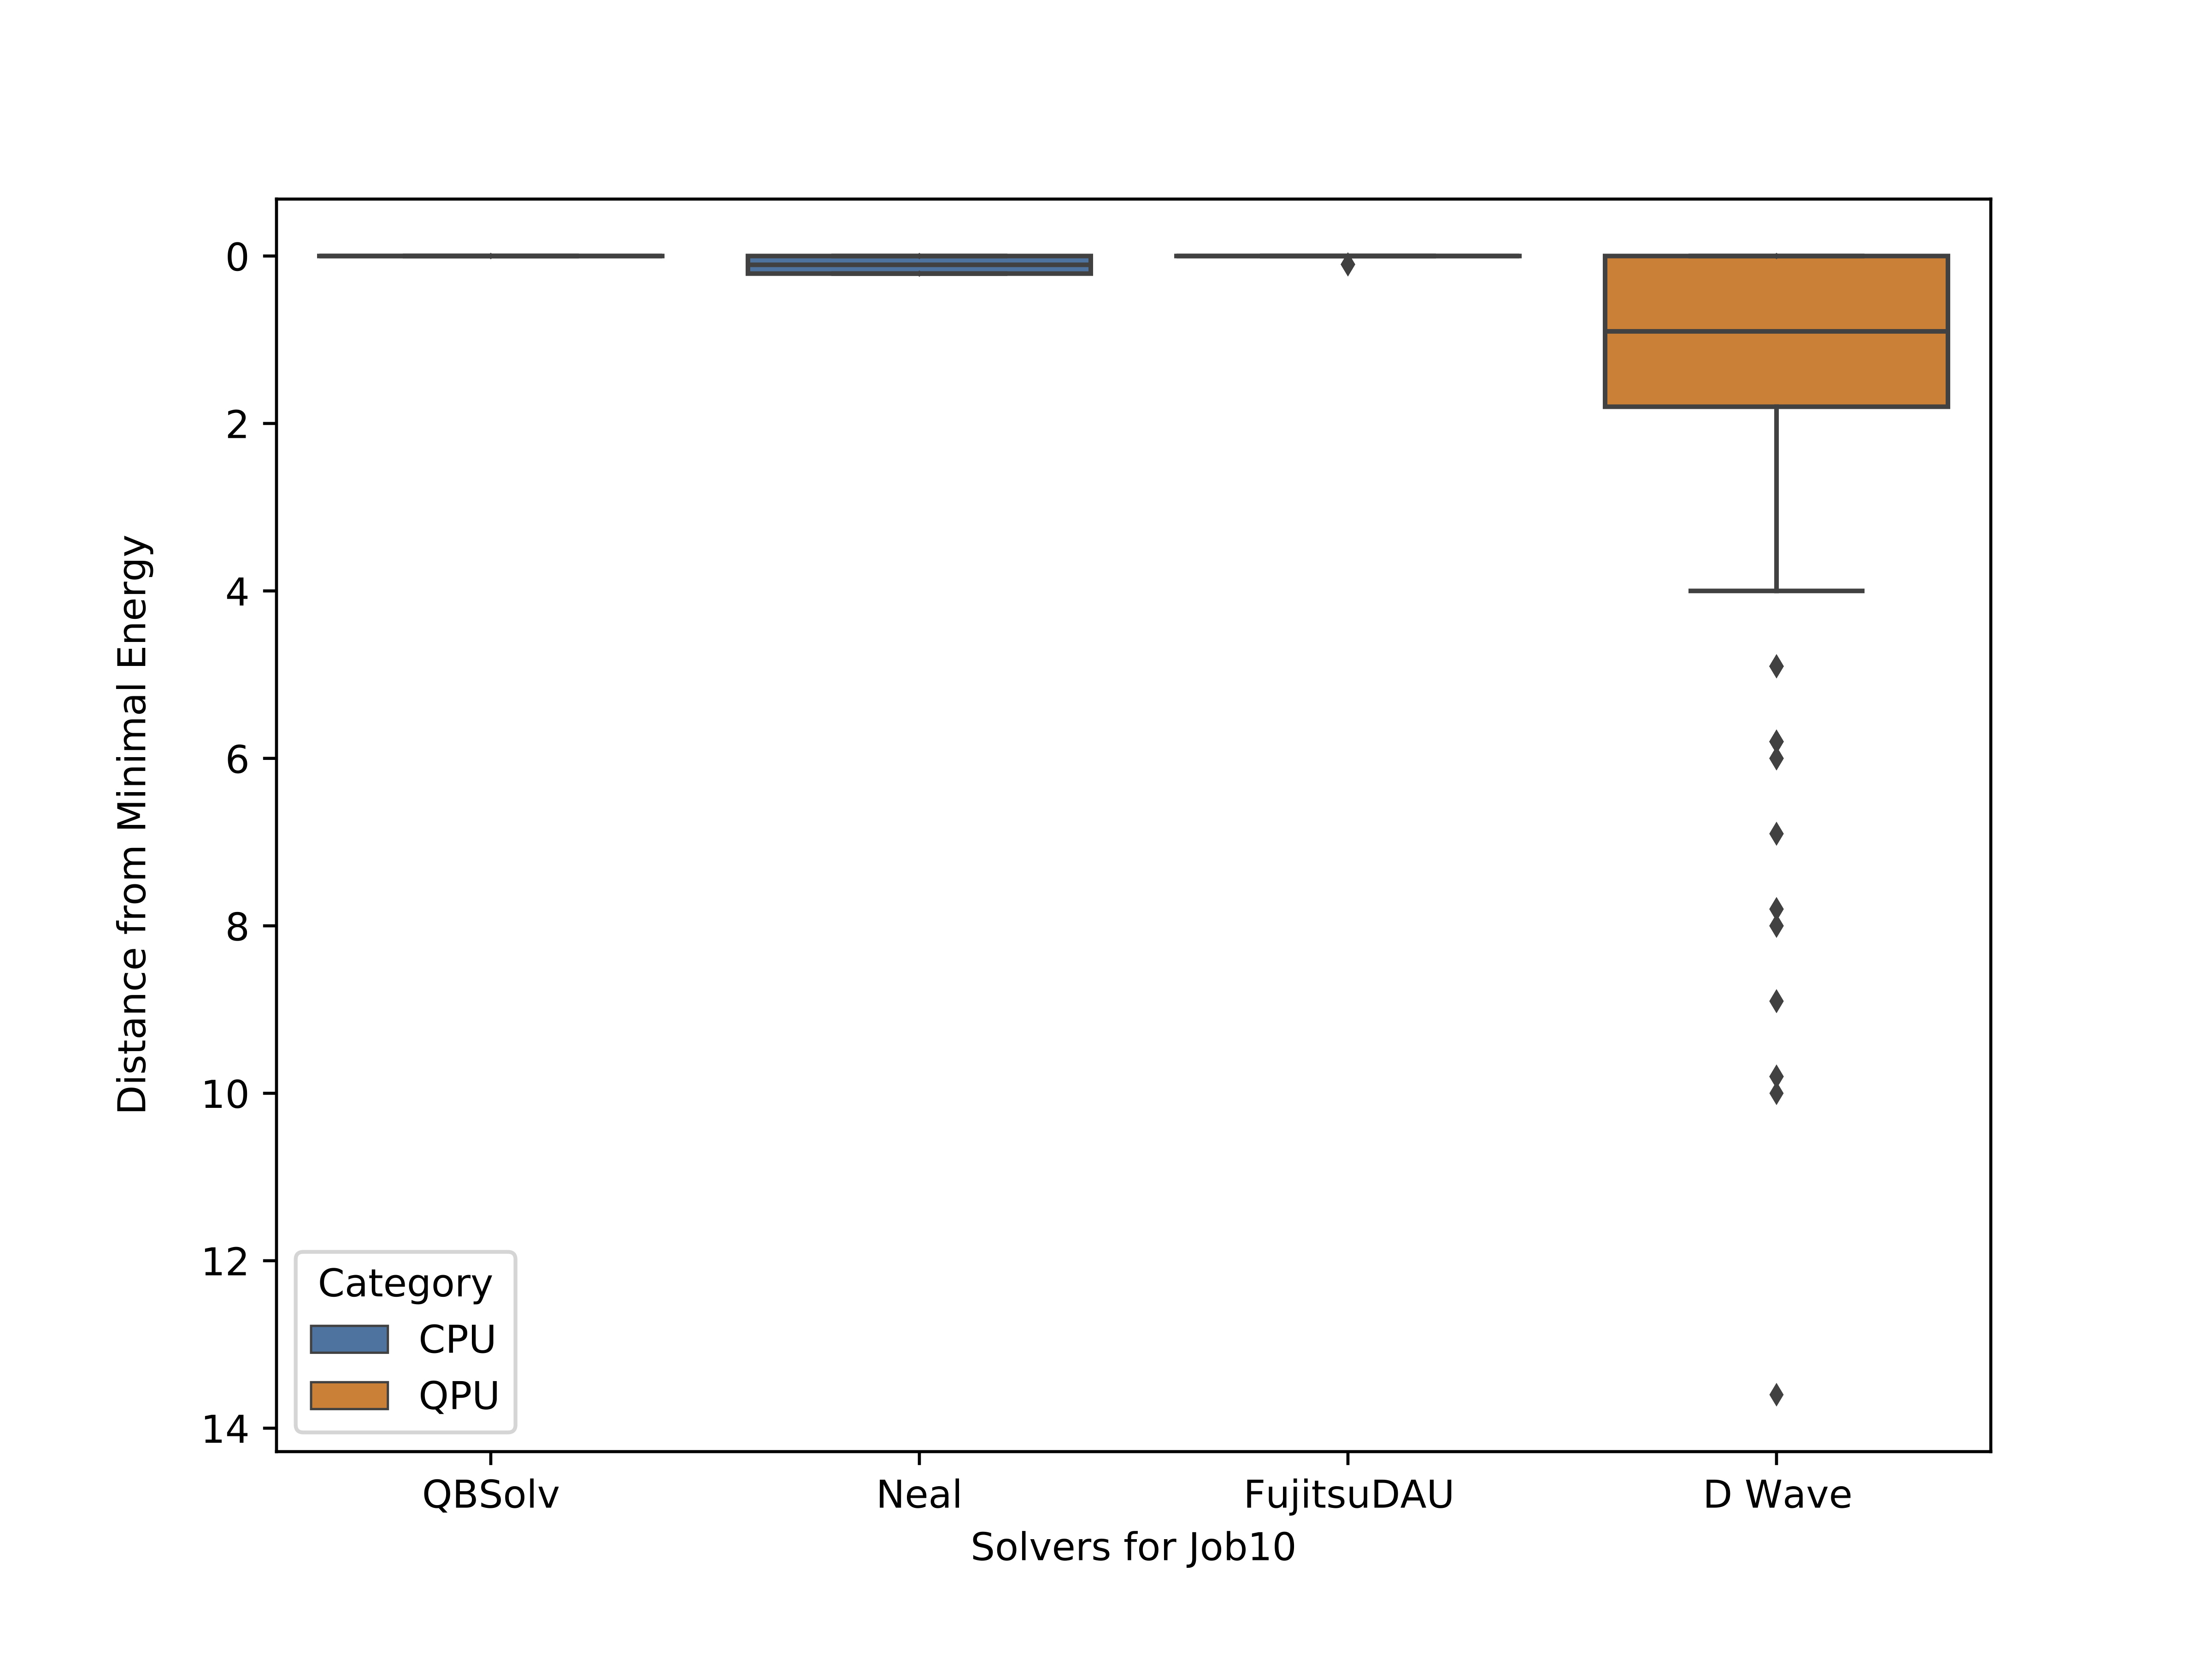
\includegraphics[width=\textwidth]{images/SolversJob10.png}
            \caption[]%
            {{\small Solver Abweichungen für Job10}}    
            \label{fig:DeviationJob10}
        \end{subfigure}
        \hfill
        \begin{subfigure}[b]{0.495\textwidth}  
            \centering 
            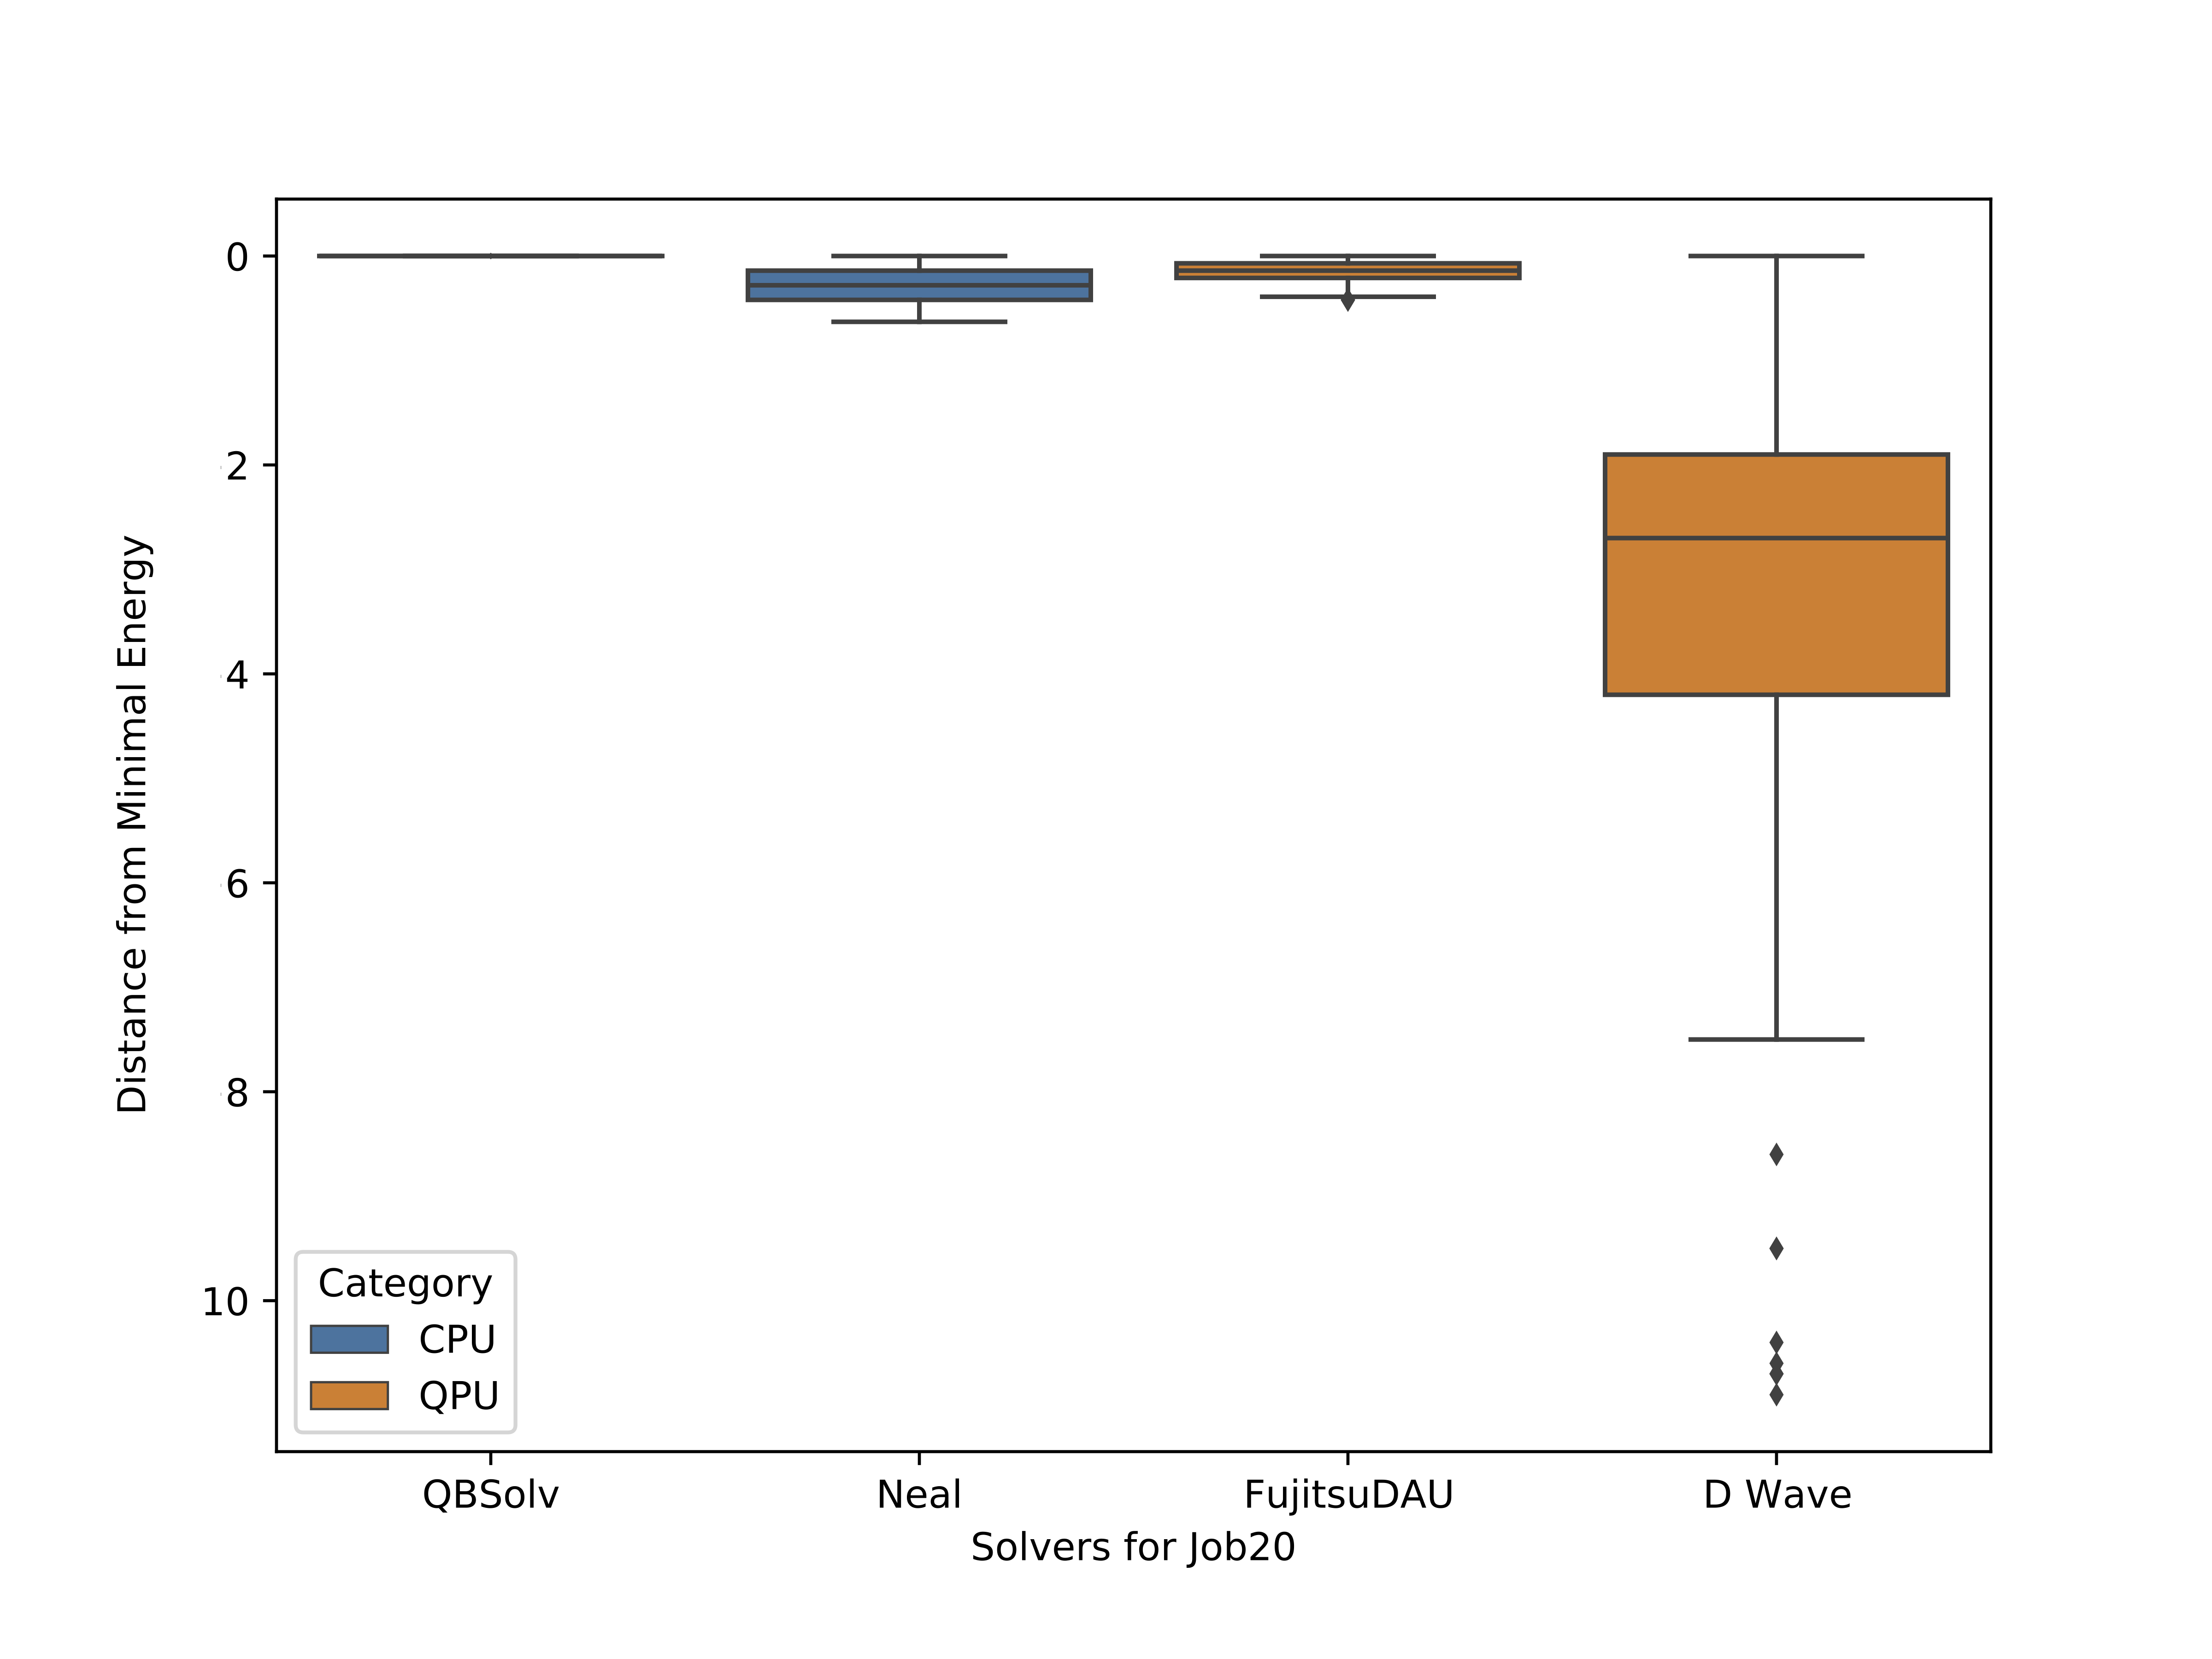
\includegraphics[width=\textwidth]{images/SolversJob20.png}
            \caption[]%
            {{\small Solver Abweichungen für Job20}}    
            \label{fig:DeviationJob20}
        \end{subfigure}
           \vskip\baselineskip
                   \begin{subfigure}[b]{0.495\textwidth}
            \centering
            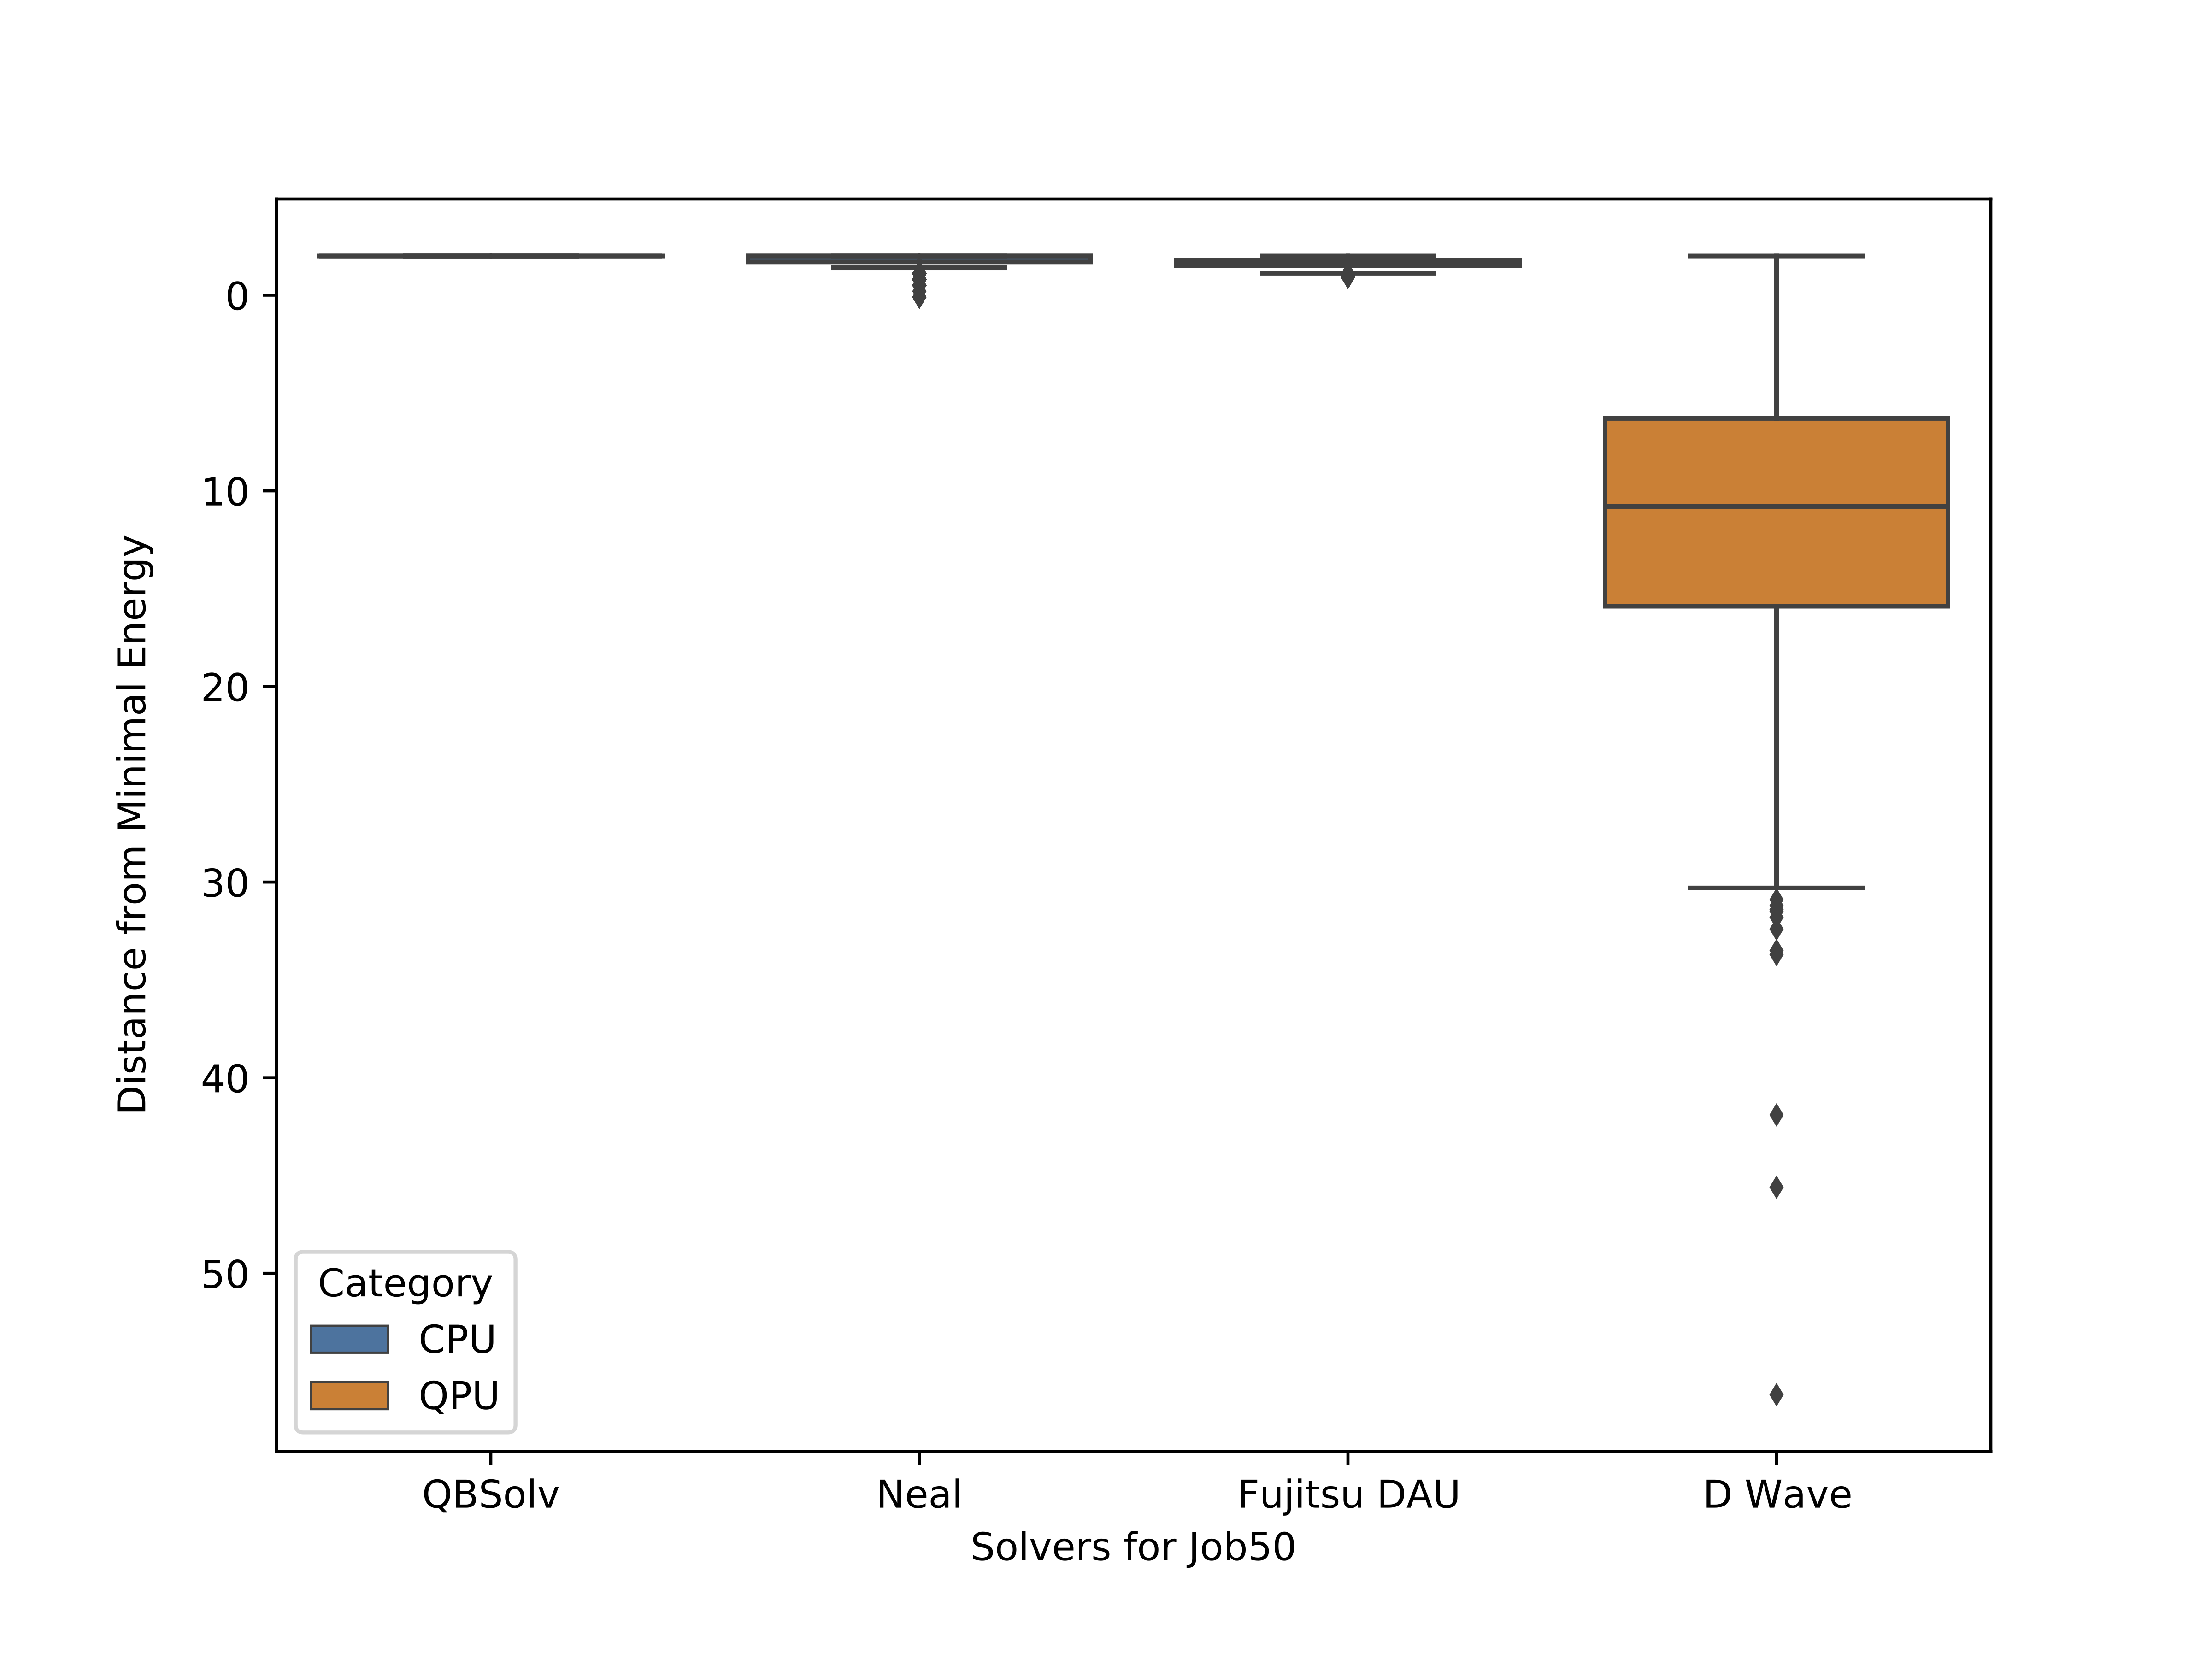
\includegraphics[width=\textwidth]{images/SolversJob50.png}
            \caption[]%
            {{\small Solver Abweichungen für Job50}}    
            \label{fig:DeviationJob50}
        \end{subfigure}
        \hfill
        \begin{subfigure}[b]{0.495\textwidth}  
            \centering 
            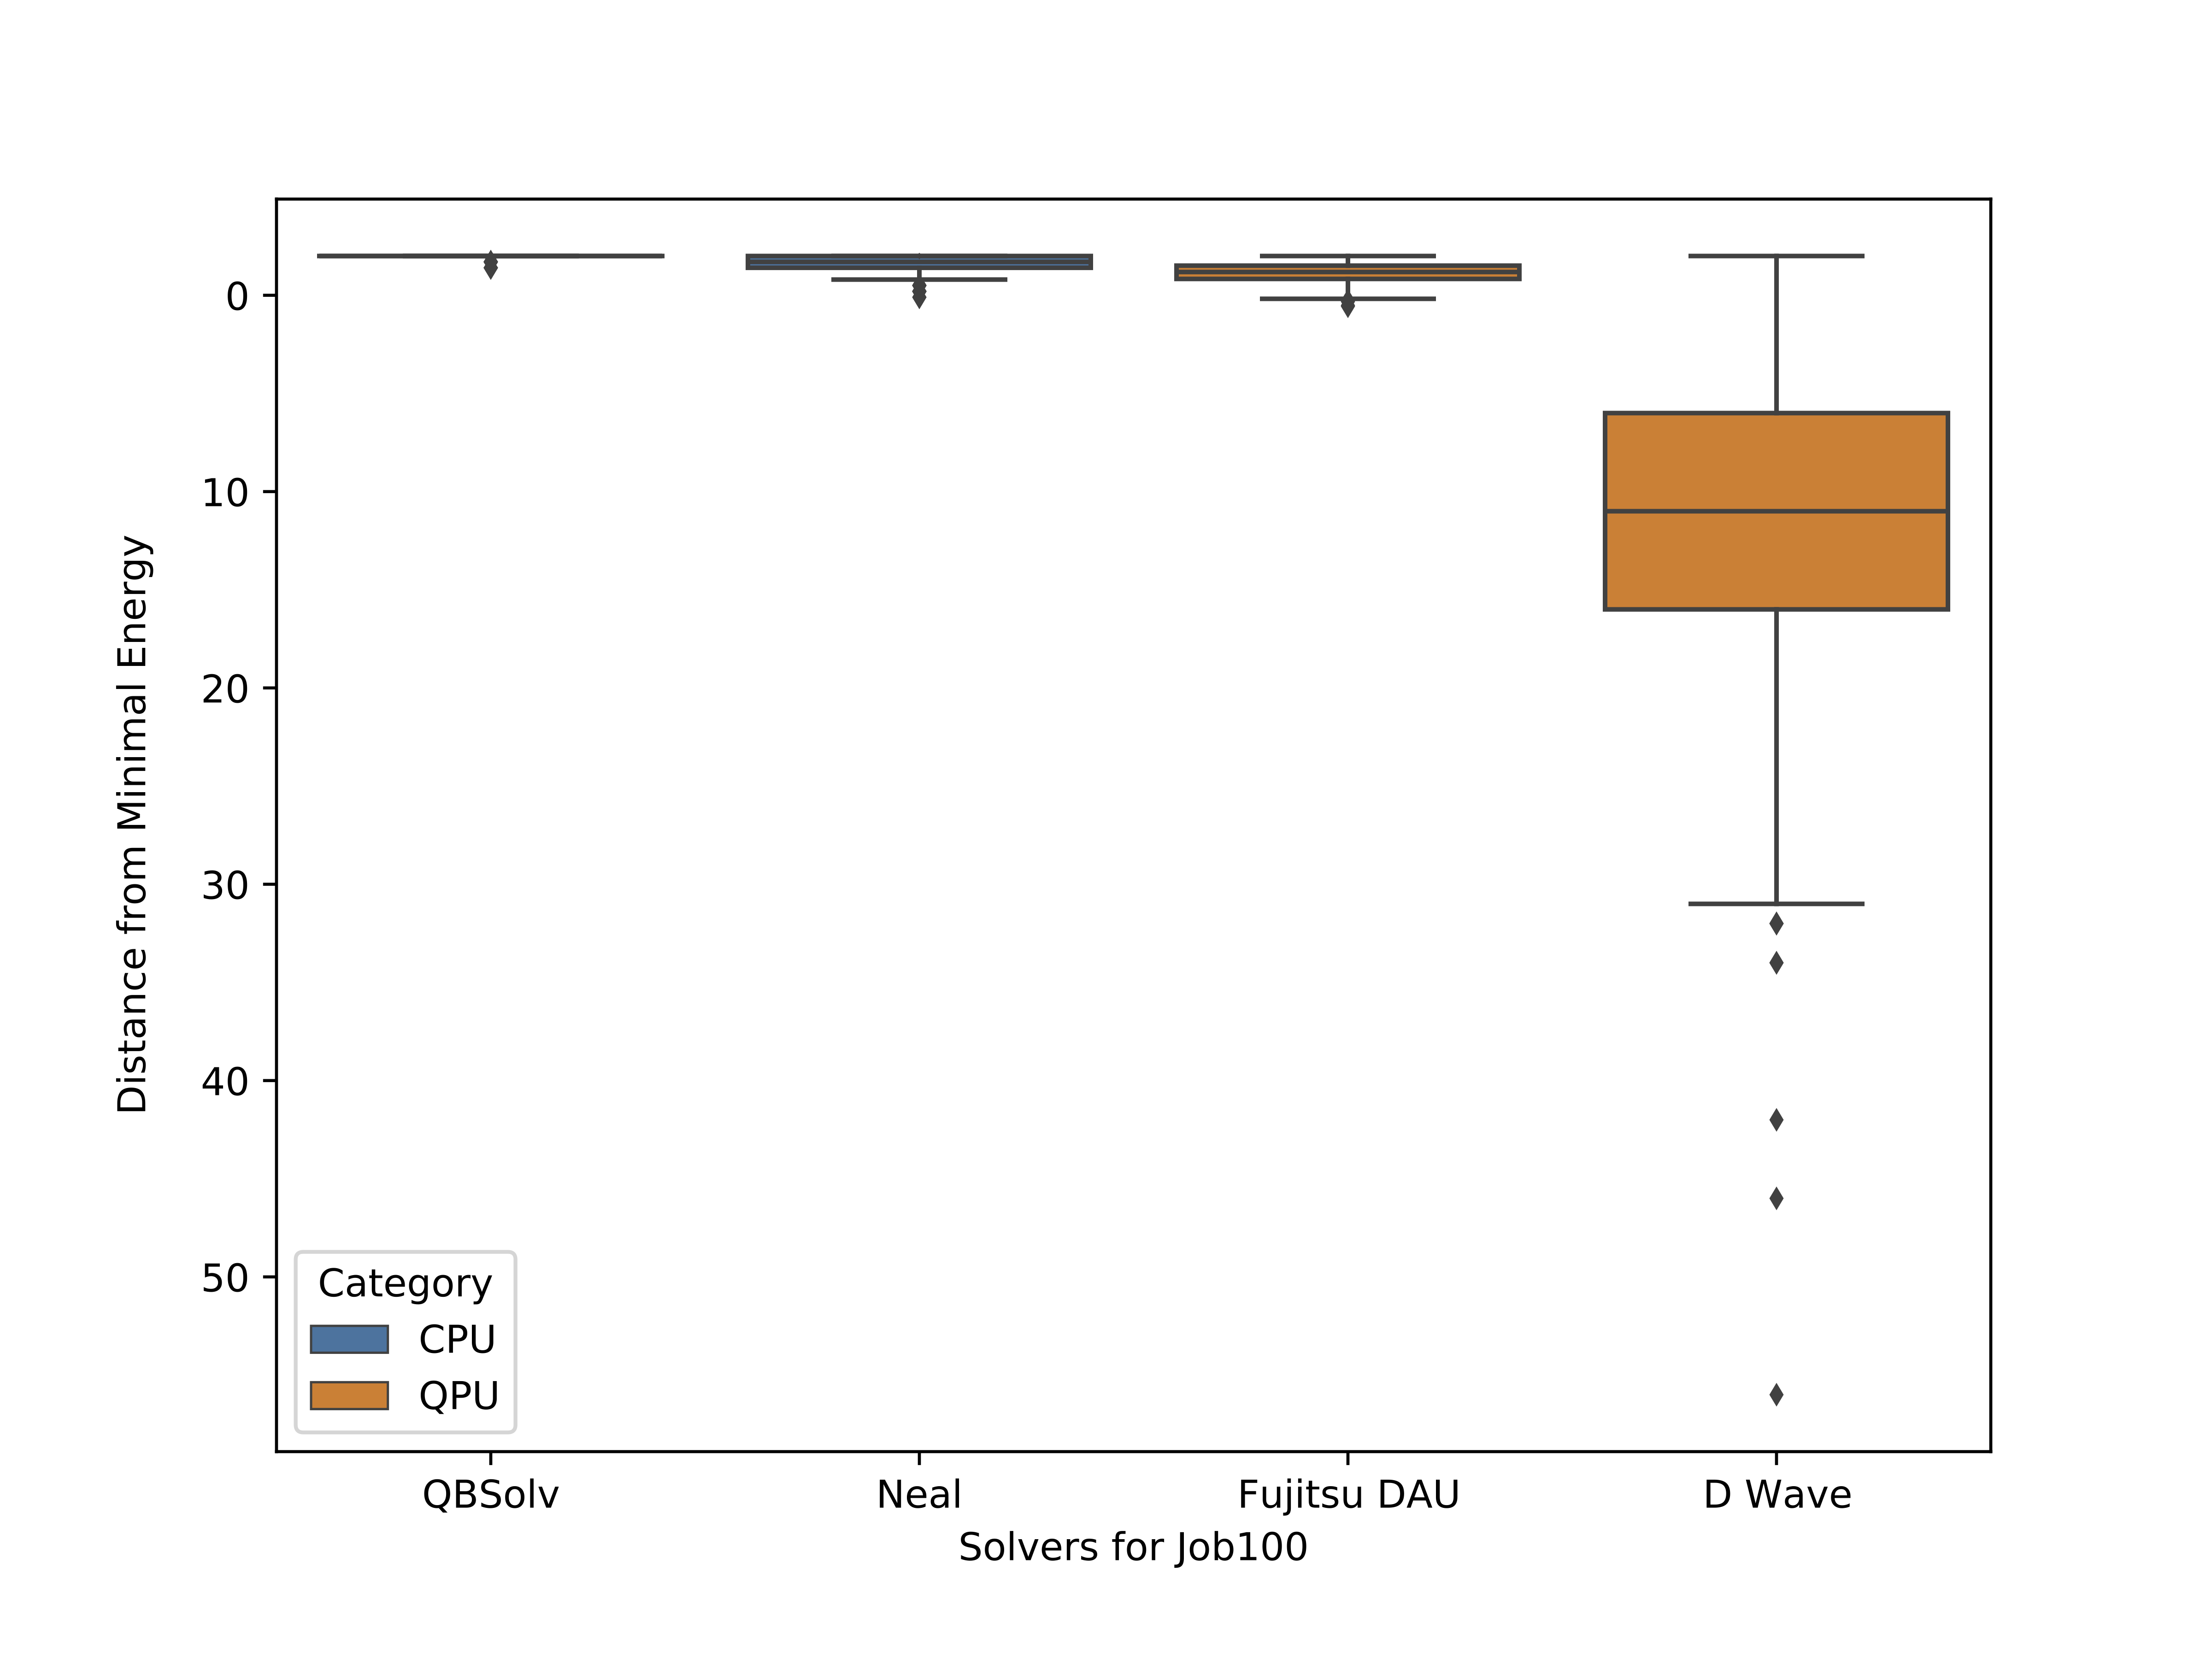
\includegraphics[width=\textwidth]{images/SolversJob100.png}
            \caption[]%
            {{\small Solver Abweichungen für Job100}}    
            \label{fig:DeviationJob100}
        \end{subfigure}
        \caption[ Ergebnisse nach Komplexität ]
         {\small Alle  Abweichungen vom Energie-Minimum ( $\widehat{=}~0$ ) nach  Solver-Art für Job10, Job20, Job50 und Job100} 
        \label{fig:B}
    \end{figure}
    
    \subsection*{Weitere Grafiken}
     \begin{figure}[H]
        \centering
        \begin{subfigure}[b]{0.4\textwidth}
            \centering
            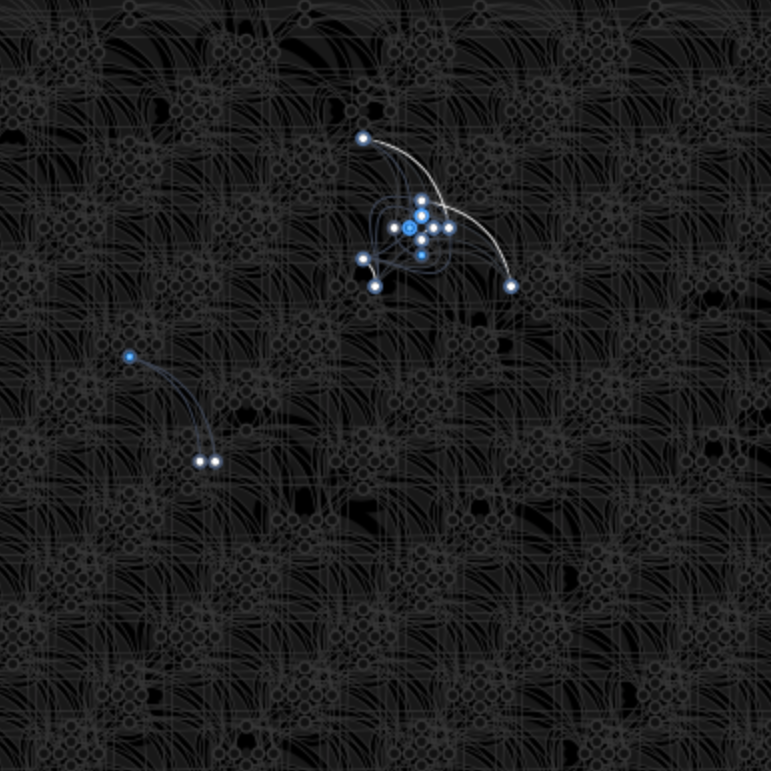
\includegraphics[width=\textwidth]{images/Embedding10.png}
            \caption[]%
            {{\small Embedding für Job10}}    
            \label{fig:EmbeddingJob10}
        \end{subfigure}
        \hfill
        \begin{subfigure}[b]{0.4\textwidth}  
            \centering 
            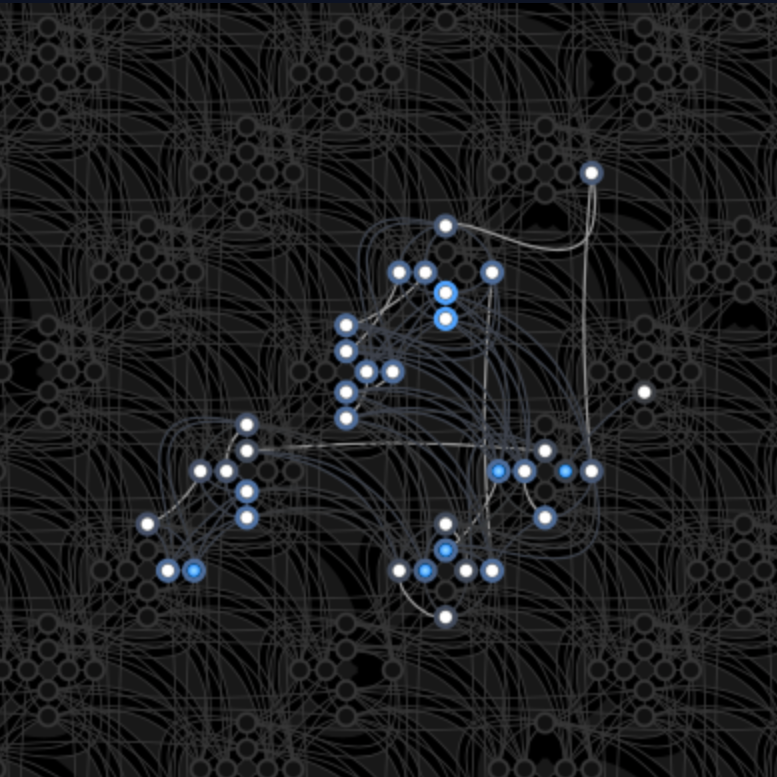
\includegraphics[width=\textwidth]{images/Embedding20.png}
            \caption[]%
            {{\small Embedding für Job20}}    
            \label{fig:EmbeddingJob20}
        \end{subfigure}
           \vskip\baselineskip
                   \begin{subfigure}[b]{0.4\textwidth}
            \centering
            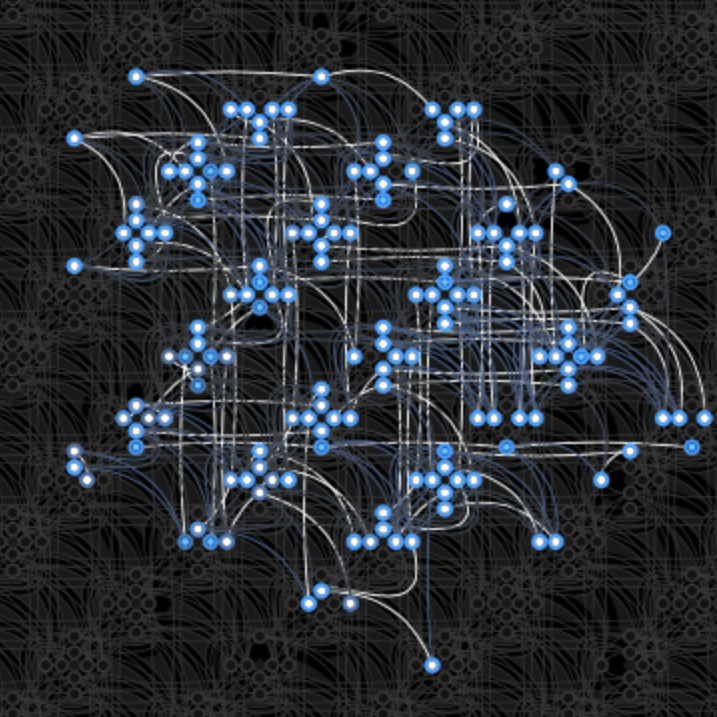
\includegraphics[width=\textwidth]{images/Embedding50.png}
            \caption[]%
            {{\small Embedding für Job50}}    
            \label{fig:EmbeddingJob50}
        \end{subfigure}
        \hfill
        \begin{subfigure}[b]{0.4\textwidth}  
            \centering 
            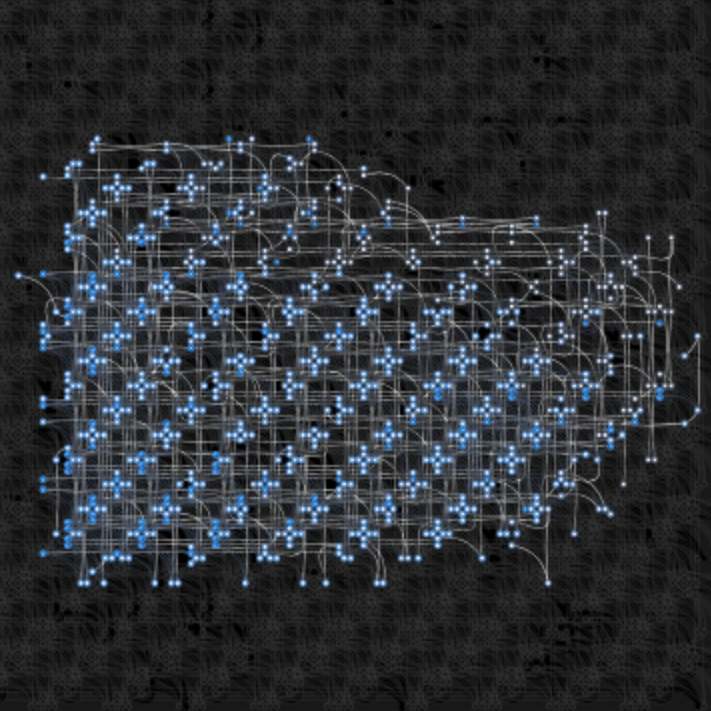
\includegraphics[width=\textwidth]{images/Embedding100.png}
            \caption[]%
            {{\small Embedding für Job100}}    
            \label{fig:EmbeddingJob100}
        \end{subfigure}
        \caption[ Ergebnisse nach Komplexität ]
         {\small Embeddings mit der besten Performance für Job10, Job20, Job50 und Job100} 
        \label{fig:B}
    \end{figure}



